\documentclass[	
	utf8,%     More capable input encoding than latin-1.
	parskip,%  For vertical whitespace between paragraphs.  This comes down to more than just using parskip.sty, so it's better to use this class option.
	% S5MP % If you intend to really use margin paragraphs (not recommended!).
	%  crop,%     Produce output with crop marks and paper size A4.  Liu-Tryck should like this.  Automatically adds information, including the physical page number, at the top of each page.
	%     Add option 'noInfo' to suppress the info at the top of each page when using option 'crop'.
	% Font options: 'kp' (default), 'times', 'lm'.  The KpFonts (loaded using 'kp'), is the most complete font among the provided options.  Among other, it supports slanted small caps.  See rtthesis.cls for more details regarding the font options.
	largesmallcaps,intlimits,widermath,% Good options to KpFonts.
	sharecounter,nobreak,definition=marks,%  See comments in the results chapter of this document for more information on these options!
	article,
	numbers, % If you want to cite references by numbers, use this option.
	noparts % Use option 'noparts' if you do not make use of part divisions.
%  tikz % Plotting.
]{rtthesis}
\usepackage{etex}

\usepackage{graphicx}
\usepackage{standalone}
\usepackage{mythesis}
\usepackage{amsthm}
\usepackage{amsmath}
\usepackage{multirow}
\usepackage{tikz}
\usepackage{ctable}
\usepackage{transparent}
\usepackage{listings}
\usepackage{framed}

\usetikzlibrary{
	fit,
	calc,
	positioning,
	circuits.ee.IEC,
	arrows,
	arrows.meta,
	patterns}

% Patch for ctable Error
\makeatletter
\begingroup\expandafter\expandafter\expandafter\endgroup
\expandafter\ifx\csname pgfutil@addpdfresource@extgs\endcsname\relax
\else
  \AtBeginDocument{%
    %\pgf@sys@addpdfresource@extgs@plain{%
    \pgfutil@addpdfresource@extgs{%
      \TRP@list
    }%
  }%  
  \let\TRP@addresource\relax
\fi
\makeatother
% End of patch

\begin{document}
\selectlanguage{english}
\makeFrontPage
\frontmatter
\maketitle
\makeLibraryPage{The computational capacity of graphics cards for general-purpose computing have been progressing fast over the last decade. A major reason is demanding computer games, where standard of performance and high quality graphics are constantly raised. Another reason are better suitable technologies for programming the graphics cards. Combined, the product are high raw performance devices and means to access that performance. This thesis investigates some of the current technologies for general-purpose computing on graphics processing units. Technologies are primarily compared by means of benchmarking performance and secondarily by factors concerning programming and implementation. The selection of technology can have a large impact on performance. The benchmark application found the difference of the fastest technology, CUDA, compared to the slowest, OpenCL, to be twice as long execution time. The application also found out that the older technologies, OpenGL and DirectX, are competitive with CUDA and OpenCL in terms of the resulting performance speed.%151
%
%En sammanfattning ska kort och koncist beskriva och motivera det studerade problemet, metoden samt resultat och slutsatser. Arbetets bidrag till huvudområdet ska tydligt framgå. Vad är det rapporten säger om huvudområdet som vi inte visste tidigare? Exempel på bidrag kan vara vilken effekt en specifik algoritm eller programutvecklingsmetod får i en specifik tillämpning.
%
%Normalt ska en sammanfattning vara högst 150 ord, och inte innehålla några referenser eller radbrytningar.
%
%Sammanfattning på svenska såväl som engelska (abstract) måste finnas med. Om rapporten är skriven på engelska räcker det med engelsk sammanfattning }

\begin{abstract}[english]
  The computational capacity of graphics cards for general-purpose computing have been progressing fast over the last decade. A major reason is demanding computer games, where standard of performance and high quality graphics are constantly raised. Another reason are better suitable technologies for programming the graphics cards. Combined, the product are high raw performance devices and means to access that performance. This thesis investigates some of the current technologies for general-purpose computing on graphics processing units. Technologies are primarily compared by means of benchmarking performance and secondarily by factors concerning programming and implementation. The selection of technology can have a large impact on performance. The benchmark application found the difference of the fastest technology, CUDA, compared to the slowest, OpenCL, to be twice as long execution time. The application also found out that the older technologies, OpenGL and DirectX, are competitive with CUDA and OpenCL in terms of the resulting performance speed.%151
%
%En sammanfattning ska kort och koncist beskriva och motivera det studerade problemet, metoden samt resultat och slutsatser. Arbetets bidrag till huvudområdet ska tydligt framgå. Vad är det rapporten säger om huvudområdet som vi inte visste tidigare? Exempel på bidrag kan vara vilken effekt en specifik algoritm eller programutvecklingsmetod får i en specifik tillämpning.
%
%Normalt ska en sammanfattning vara högst 150 ord, och inte innehålla några referenser eller radbrytningar.
%
%Sammanfattning på svenska såväl som engelska (abstract) måste finnas med. Om rapporten är skriven på engelska räcker det med engelsk sammanfattning 
\end{abstract}
\begin{acknowledgments}%
	I would like to thank Åsa Detterfelt for the opportunity to make this thesis work at MindRoad AB. I would also like to thank Ingemar Ragnemalm at ISY.
	
	\addvspace{1em}%
	\begin{flushright}%
    \textit{%
		Linköping, Februari 2016 \\%
		Torbjörn Sörman%
	}%
	\end{flushright}%
	
\end{acknowledgments}%

\tableofcontents
\begin{notation}% Passing the option "old" to the notation environment will redefine the notationtabular environment so that it produces an old style LaTeX tabular instead of a ctable.sty style tabular.
	\centering
	
	\begin{notationtabular}{Glossary}{Term}{Meaning}
		Kernel & A \gls{GPU} program \\
		Thread & A way for a program to split itself to many simultaneously running tasks \\
		Block & A way to organize threads, a block is executed by a multiprocessing unit \\
	\end{notationtabular}

\end{notation}


\mainmatter
\chapter{Introduction}\label{cha:intro}
This chapter gives an introduction to the thesis. It describes the background, purpose and goal of the thesis, and also a list of abbreviations and the structure of this report.

\section{Background}
The computationally demanding problems have during a long period of time been solved faster by technical improvements in hardware. However, some limitations have been reached the last decades. Operating frequency of the \gls{CPU} is no longer significantly improved. Problems relying on single thread performance are limited by three primary technical factors:
\begin{enumerate}
	\item The \gls{ILP} wall
	\item The memory wall
	\item The power wall
\end{enumerate}

The first wall states that its hard to further exploit simultanious \gls{CPU} instructions, techniques like instruction pipelining, superscalar execution and \gls{VLIW} exists but complexity and latency of hardware reduces the benefits. Related to the first is second wall, the gap between \gls{CPU} speed and memory access time, that may cost several hundreds of \gls{CPU} cykles if accessing primary memory. The third wall is power and heating problem. The power consumed is increased exponentially with each factorial increase of operating frequency.

Improvements can be found in exploiting parallelism. Either reconstruct the problem or the problem itself is already inherently parallelizable. This trend manifests in development towards use and construction of multi-core microprocessors. The \gls{GPU} is one such device, originally exploited the inherent parallelism within visual rendering but now is available as a tool for massively parallelizable problems.

\section{Problem statement}
Programmers might experience a threshold and slow learning curve to move from sequential to thread-parallel programming that is \gls{GPU} programming. Obstacles involve learning about the hardware architecture and restructure the application. Knowing limitations and benefits might even provide reason to not utilize the \gls{GPU} and instead choose to work with a multi-core \gls{CPU}.

Depending on one's preferences, needs and future goals; selecting one technology over the other might be derived from portability or hardware requirements, programmability, how well it integrates with other frameworks or \gls{API} or how well it's supported by the provider or developer community. Within the range of this thesis, the covered technologies are \gls{CUDA}, \gls{OpenCL}, DirectCompute (\gls{API} within DirectX) and \gls{OpenGL} Compute Shaders.

\section{Purpose and goal of the thesis work}
One goal is to evaluate, select and implement an application suitable for \gls{GPGPU}.

Implement the same application in important technologies for \gls{GPGPU}:
\begin{itemize}
	\item \CU
	\item \OCL
	\item \DX
	\item \GL
\end{itemize}
Compare results with sequential {\CPP} implementation and an multi-core {\OMP} implementation.

The purpose is to compare the different technologies by means of benchmarking performance and make relevant qualitative assessments.
\chapter{Technologies}

Five different multi-core technologies are used in this study. One is specialized in GPGPU, namely CUDA. OpenGL and DirectCompute are parts of graphic programming languages but breaks away from the graphics abstraction with \textit{Compute Shaders}. OpenCL aims at any heterogeneous multi-core system and is used in this study to use on the GPU. To compare with the CPU, OpenMP is included as a fast and easy way to parallelize C/C++ -code.

\section{CUDA}

CUDA is an acronym for Compute Unified Device Architecture, developed by NVIDIA and released in 2006. CUDA is an extension of the C/C++ language and have its own compiler. CUDA supports the functionality to execute kernels, modify the graphic card RAM memory and the use of several optimized function libraries such as \textit{cuBLAS} (CUDA implementation of BLAS, Basic Linear Algebra Subprograms) or \textit{cuFFT} (CUDA implementation of FFT).

A program running on the GPU is called a kernel. The GPU is referred to as the \textit{device} and the the CPU is called the \textit{host}. To run a CUDA kernel all that is needed is to declare the program with a function type specifier, see table \ref{tab:cuda:func-types}, and call it from the host with launch parameters.

\begin{table}
	%\includestandalone[width=\textwidth]{tables/cuda-function-types}
	\centering
	%\begin{tabular}{|l|l|l|}
	\hline
	Function type & Executed on & Callable from \\ \hline
	\texttt{\_\_device\_\_} & Device & Device \\ \hline
	\texttt{\_\_global\_\_} & Device & Host \\ \hline
	\texttt{\_\_host\_\_} & Host & Host \\ \hline
\end{tabular}
	\caption{Table of function types in CUDA.}
	\label{tab:cuda:func-types}
\end{table}

\begin{figure}
	\centering
	\lstset{language=C++}
	\begin{framed}
	\begin{lstlisting}
// Device program (GPU)
__global__ void myKernel(float val)
{
  int tid = threadIdx.x + blockDim.x * blockIdx.x;
}

// Host program (CPU)
__host__ void myFunction(float value)
{
  dim3 threads = {1024, 1, 1};
  dim3 blocks  = {1, 1, 1};
  myKernel<<<blocks, threads>>>(value);
}
	\end{lstlisting}
	\end{framed}
\end{figure}

\section{OpenCL}

\section{DirectCompute}

\section{OpenGL Compute Shader}

\section{OpenMP}
\chapter{Theory}

This chapter will give an introduction to the FFT algorithm and a brief introduction of the Graphics Processing Unit (GPU).

\section{Graphics Processing Unit}

A GPU is traditionally specialized hardware for efficient manipulation of computer graphics and image processing. The inherent parallel structure of images and graphics makes them very efficient at some more general problems where parallelism can be exploited. The concept of General-purpose computing on graphics processing units (GPGPU) is solving a problem on the GPU platform instead of a multi-core CPU system.

\subsection{GPGPU}

In the early days of GPGPU one had to know a lot about computer graphics to compute general data. The available APIs was created for graphics processing. The dominant APIs was OpenGL and DirectX. HLSL (High Level Shader Language) and GLSL (OpenGL Shader Language) made the step easier but it still generated code into the APIs.

A big change was when NVIDIA released {\CU} and together with new hardware made it possible to use standard C-code to program the GPU (with a few extensions). The fact that parallel software and hardware was a small market at the time, the simplified use of the GPU for parallel tasks opened up to many more customers. However, the main business is still graphics and the manufacturers can not make cards too expensive, especially at the cost of graphics performance (as integrating more double precision capacity would). This can be exemplified with the release of NVIDIA's Maxwell micro architecture, compared to the predecessor Kepler, both are similar but with Maxwell some of the double precision support was removed in favour of single precision (used in graphics).

\subsection{GPU vs CPU}

The GPU is built on a principle of more execution units instead of higher clock-frequency to improve performance. Comparing the CPU with the GPU, the GPU performs a much higher floating point operations per second (FLOP) if running at optimal conditions. The GPU relies on using high memory bandwidth and fast context switching (run the next warp of threads) to compensate for lower frequency and hide memory latencies. The CPU is excellent at sequential tasks with features like branch prediction that can not be found on the GPU.

The GPU thread is very lightweight and its creation have very little overhead, whereas on the CPU the thread can be seen as an abstraction of the processor and switching a thread is considered expensive since the context have to be loaded each time. On the other hand, a GPU is very inefficient if not enough threads are ready to work. Memory latencies are supposed to be hidden by switching in a new set of working threads as fast as possible.

A CPU thread have its own registers but the GPU thread work in groups where they share registers and memory. One can not give individual instructions to each thread, all of them will execute the same instruction. The figure \ref{fig:gpu-vs-cpu} demonstrates this by showing that by sharing control-structure and cache, the GPU puts more resources on processing then the CPU where more resources goes into control structures and memory cache.

\begin{figure}
	\centering
	\includestandalone[width=\textwidth]{figures/gpu-cpu}
	\caption{The GPU uses more transistors for data processing}
	\label{fig:gpu-vs-cpu}
\end{figure}

\section{Fast Fourier Transform}

This section extends the information from section \ref{sec:algorithms:fft} in the \textit{Benchmark application} chapter.

\subsection{\CTALG}

The Fast Fourier Transform is by far mostly associated with the {\CTALG} algorithm. The {\CTALG} algorithm is a devide and conquer algorithm that recursively breaks down a DFT of any composite size of $N = N_1{\cdot}N_2$. The algorithm decomposes the DFT into $s = \log_r{N}$ stages. The $N$-point DFT is composed of $r$-point small DFTs in $s$ stages. In this context the $r$-point DFT is called radix-$r$ butterfly.

\subsubsection{Butterfly and radix-2}

The implementation of a $N$-point radix-2 FFT algorithm have $\log_2{N}$ stages with $N/2$ butterfly operations per stage. A butterfly operation is an addition, a subtraction, followed by a multiplication by a twiddle factor, see figure \ref{fig:butterfly}.

\begin{figure}
	\centering
	% FFT Butterfly
\tikzstyle{n}= [circle, fill, minimum size=4pt,inner sep=0pt, outer sep=0pt]
\tikzstyle{mul} = [circle,draw,inner sep=-1pt, minimum size=7pt]
\tikzstyle{sub} = [circle,draw,inner sep=-1pt, minimum size=7pt]
\tikzstyle{add} = [circle,draw,inner sep=-1pt, minimum size=7pt]

\begin{tikzpicture}[
	yscale=1.3,
	xscale=1.8,
	node distance=0.7cm,
	auto]
    
	\node[n, pin={[pin edge={latex'-,black}]left:$x(0)$}] (N-0-0) at (0,-0) {};
	\node[n, pin={[pin edge={latex'-,black}]left:$x(1)$}] (N-0-1) at (0,-1) {};
                            
	\node[add, name=N-1-0, pin={[pin edge={-latex',black},pin distance=1.175cm]right:$X(0)$}] at (1,-0) {${+}$};
	\node[sub, name=N-1-1, label={[label distance=-10pt]90:${-}$}] at (1,-1) {};
            
	\node[mul, right of=N-1-1, label={above right:\tiny $W^{k}_{N}$},
		pin={[pin edge={-latex',black}]right:$X(1)$}] (N-2-1) {${\times}$};       

	\path (N-0-0) edge[-latex'] (N-1-0);	
	\path (N-0-1) edge[-latex'] (N-1-1);
	\path (N-1-1) edge[-latex'] (N-2-1);
      
    % Connect nodes
    \foreach \src / \dst in {	0/0, 0/1, 1/0, 1/1}
       \path (N-0-\src.east) edge[-latex'] (N-1-\dst.west);
       
\end{tikzpicture}
	\caption{Radix-2 butterfly operations}
	\label{fig:butterfly}
\end{figure}

Figure \ref{fig:cooley-tukey-8} shows an 8-point radix-2 DIF FFT. The input are in natural order whereas the output are in bit reversed order.

\begin{figure}
	\centering
	% FFT Butterfly
\tikzstyle{n}= [circle, fill, minimum size=4pt,inner sep=0pt, outer sep=0pt]
\tikzstyle{mul} = [circle,draw,inner sep=-1pt]

% Define two helper counters
\newcounter{x}\newcounter{y}
\begin{tikzpicture}[%
	%yscale=0.6,
	%xscale=1.2,
	node distance=0.25cm,
	auto]
    % Draw inputs
    \foreach \y in {0,...,7}
        \node[n, pin={[pin edge={latex'-,black}]left:$x(\y)$}] (N-0-\y) at (0,-\y) {};

	\foreach \y in {0,...,7}
        \foreach \x / \c in {1/1,2/3,3/4,4/6,5/7,6/9}
            \node[n, name=N-\c-\y] at (\x,-\y) {};           
    
    % Draw outputs
    \foreach \y in {0,...,7}
        \node[n, pin={[pin edge={-latex',black}]right:$X(\y)$}] (N-11-\y) at (8,-\y) {};
        
    % horizontal connections
    % Note the use of simple counter arithmetics to get correct
    % indexes.
    \foreach \y in {0,...,15}
    {
		\foreach \x in {0,1,3,4,7}
		{
			\setcounter{x}{\x}\stepcounter{x}
			\path (N-\x-\y) edge[-] (N-\arabic{x}-\y);
		}
	}
           
    % Draw the W_8 coefficients
    \setcounter{y}{0}
    \foreach \tmp in {0,1}
	{
    	\foreach \i in {0,...,3}
    	{
        	\path (N-5-\arabic{y}) edge[-] node {} (N-6-\arabic{y});
        	\addtocounter{y}{1}
    	}
    }

    % Draw the W_4 coefficients
    \setcounter{y}{0}
    \foreach \tmp in {0,1}
	{
    	\foreach \i in {0,1}
    	{
        	\path (N-5-\arabic{y}) edge[-] node {} (N-6-\arabic{y});
        	\addtocounter{y}{1}
    	}
    	\foreach \i in {0,1}
    	{
        	\path (N-5-\arabic{y}) edge[-] node {\tiny $W^{\i}_{8}$} (N-6-\arabic{y});
        	\addtocounter{y}{1}
    	}
    }
    
    % Connect nodes
    \foreach \sourcey / \desty in {	0/4,	1/5,	2/6,	3/7,
									4/0,	5/1,	6/2,	7/3}
        \path (N-3-\sourcey.east) edge[-] (N-4-\desty.west);
    \foreach \sourcey / \desty in {	0/0,	1/2,	2/0,	3/2,
    								0/1,	1/3,	2/1,	3/3,
                                   	4/4,	5/6,	6/4,	7/6,
                                   	4/5,	5/7,	6/5,	7/7,}
	{
        \path (N-6-\sourcey.east) edge[-] (N-7-\desty.west);
        \path (N-9-\sourcey.east) edge[-] (N-10-\desty.west);
    }
    
    % Add region boxes	
    % Complete stage
	\node[draw,densely dotted,fit=(N-0-0) (N-2-15),label=above:{stage 1}] {};
	\node[draw,densely dotted,fit=(N-3-0) (N-5-15),label=above:{stage 2}] {};
	\node[draw,fit=(N-6-0) (N-8-15),opacity=0,label=above:{stage 3},name=Stage-3] {};
	\node[draw,fit=(N-9-0) (N-\lastNode-15),opacity=0,label=above:{stage 4},name=Stage-4] {};
	\node[draw,fit=(N-11-0) (N-11-15),opacity=0,label=above:{output}] {};
	\node[draw,densely dotted,fit=(Stage-3) (Stage-4)] {};
	\node[draw,fit=(N-\lastNode-0) (N-11-15)] {};
\end{tikzpicture}
	\caption{8-point radix-2 FFT using {\CTALG} algorithm}
	\label{fig:cooley-tukey-8}
\end{figure}

\subsubsection{\CGALG}

Similar to {\CTALG} but with another data access pattern that uses the same indexing in all stages. This removes the overhead of calculating the data input index at each stage as in figure \ref{fig:cooley-tukey-8} where the top butterfly first stage require input $x[0], x[4]$ and in the second stage $x[0], x[2]$ whereas using the {\CGALG} algorithm in figure \ref{fig:constant-geometry-8} the equivalent input are $x[0], x[4]$ for all stages.

\begin{figure}
	\centering
	% FFT Butterfly
\tikzstyle{n}= [circle, fill, minimum size=4pt,inner sep=0pt, outer sep=0pt]
\tikzstyle{mul} = [circle,draw,inner sep=-1pt]

% Define two helper counters
\newcounter{x}\newcounter{y}
\begin{tikzpicture}[%
	yscale=0.6,
	xscale=1.2,
	node distance=0.25cm,
	auto]
    % The strategy is to create nodes with names: N-column-row
    % Input nodes are named N-0-0 ... N-0-15
    % Output nodes are named N-10-0 ... N-10-15

    % Draw inputs
    \foreach \y in {0,...,15}
        \node[n, pin={[pin edge={latex'-,black}]left:$x(\y)$}] (N-0-\y) at (0,-\y) {};
              
    % Draw outputs
    \foreach \y in {0,...,15}
        \node[n, pin={[pin edge={-latex',black}]right:$X(\y)$}] (N-11-\y) at (8,-\y) {};
              
   % draw connector nodes
    \foreach \y in {0,...,15}
        \foreach \x / \c in {1/1,2/3,3/4,4/6,5/7,6/9,7/10}
            \node[n, name=N-\c-\y] at (\x,-\y) {};
            
    % draw x nodes
    \foreach \y in {0,...,7}
        \foreach \x / \c  in {1/2}
            \node[mul, right of=N-\x-\y] (N-\c-\y) {};            
    \foreach \y in {8,...,15}
        \foreach \x / \c  in {1/2}
            \node[mul, right of=N-\x-\y] (N-\c-\y) {${\times}$};
    % 
    \foreach \y in {0,...,3}
        \foreach \x / \c  in {4/5}
            \node[mul, right of=N-\x-\y] (N-\c-\y) {};
    \foreach \y in {4,...,7}
        \foreach \x / \c  in {4/5}
            \node[mul, right of=N-\x-\y] (N-\c-\y) {${\times}$};
    \foreach \y in {8,...,11}
        \foreach \x / \c  in {4/5}
            \node[mul, right of=N-\x-\y] (N-\c-\y) {};
    \foreach \y in {12,...,15}
        \foreach \x / \c  in {4/5}
            \node[mul, right of=N-\x-\y] (N-\c-\y) {${\times}$};
    % 
    \foreach \y in {0,2,4,6,8,10,12,14}
        \foreach \x / \c  in {7/8}
            \node[mul, right of=N-\x-\y] (N-\c-\y) {};
    \foreach \y in {1,3,5,7,9,11,13,15}
        \foreach \x / \c  in {7/8}
            \node[mul, right of=N-\x-\y] (N-\c-\y) {${\times}$};    

    % horizontal connections
    % Note the use of simple counter arithmetics to get correct
    % indexes.
    \foreach \y in {0,...,15}
    {
		\foreach \x in {0,1,3,4,7}
		{
			\setcounter{x}{\x}\stepcounter{x}
			\path (N-\x-\y) edge[-] (N-\arabic{x}-\y);
		}
	}
       
    % Draw the W_16 coefficients
    \setcounter{y}{0}
    \foreach \i in {0,...,7}
    {
	   	\path (N-2-\arabic{y}) edge[-] node {} (N-3-\arabic{y});
	    \stepcounter{y}
    }
    \foreach \i in {0,...,7}
    {
    	\path (N-2-\arabic{y}) edge[-] node {\tiny $W^{\i}_{16}$} (N-3-\arabic{y});
        \stepcounter{y}
    }
    
    % Draw the W_8 coefficients
    \setcounter{y}{0}
    \foreach \tmp in {0,1}
	{
    	\foreach \i in {0,...,3}
    	{
        	\path (N-5-\arabic{y}) edge[-] node {} (N-6-\arabic{y});
        	\addtocounter{y}{1}
    	}
    	\foreach \i in {0,...,3}
    	{
        	\path (N-5-\arabic{y}) edge[-] node {\tiny $W^{\i}_{8}$} (N-6-\arabic{y});
        	\addtocounter{y}{1}
    	}
    }

    % Draw the W_4 coefficients
    \setcounter{y}{0}
	\foreach \tmp in {0,...,3}
	{    
		\foreach \i in {0,1}
		{
			\path (N-8-\arabic{y}) edge[-] node {} (N-9-\arabic{y});
			\stepcounter{y}
			\path (N-8-\arabic{y}) edge[-] node {\tiny $W^{\i}_{4}$} (N-9-\arabic{y});
			\stepcounter{y}
		}
    }
    
    % Connect nodes
    \foreach \sourcey / \desty in {	0/8,	1/9,	2/10,	3/11,
									4/12,	5/13,	6/14,	7/15,
									8/0,	9/1,	10/2,	11/3,
									12/4,	13/5,	14/6,	15/7}
       \path (N-0-\sourcey.east) edge[-] (N-1-\desty.west);
    \foreach \sourcey / \desty in {	0/4,	1/5,	2/6,	3/7,
									4/0,	5/1,	6/2,	7/3,
									8/12,	9/13,	10/14,	11/15,
									12/8,	13/9,	14/10,	15/11}
        \path (N-3-\sourcey.east) edge[-] (N-4-\desty.west);
    \foreach \sourcey / \desty in {	0/0,	1/2,	2/0,	3/2,
    								0/1,	1/3,	2/1,	3/3,
                                   	4/4,	5/6,	6/4,	7/6,
                                   	4/5,	5/7,	6/5,	7/7,
                                   	8/8,	9/10,	10/8,	11/10,
									8/9,	9/11,	10/9,	11/11,
									12/12,	13/14,	14/12,	15/14,
									12/13,	13/15,	14/13,	15/15}
	{
        \path (N-6-\sourcey.east) edge[-] (N-7-\desty.west);
        \path (N-9-\sourcey.east) edge[-] (N-10-\desty.west);
    }
    % Nodes are in bit-reverse order
    \foreach \sourcey / \desty in {	0/0,1/8,2/4,3/12,4/2,5/10,6,7/14,8/1,9,10/5,11/13,12/3,13/11,14/7,15/15}
	{
        \path (N-10-\sourcey.east) edge[-] (N-11-\desty.west);
    }
    
    % Add region boxes
	% Partial stage
	\def \lastNode {10}
	\node[draw,dashed,fit=(N-6-0) (N-\lastNode-3)] {};
	\node[draw,dashed,fit=(N-6-4) (N-\lastNode-7)] {};
	\node[draw,dashed,fit=(N-6-8) (N-\lastNode-11)] {};
	\node[draw,dashed,fit=(N-6-12) (N-\lastNode-15)] {};	
    % Complete stage
	\node[draw,densely dotted,fit=(N-0-0) (N-2-15),label=above:{stage 1}] {};
	\node[draw,densely dotted,fit=(N-3-0) (N-5-15),label=above:{stage 2}] {};
	\node[draw,fit=(N-6-0) (N-8-15),opacity=0,label=above:{stage 3},name=Stage-3] {};
	\node[draw,fit=(N-9-0) (N-\lastNode-15),opacity=0,label=above:{stage 4},name=Stage-4] {};
	\node[draw,fit=(N-11-0) (N-11-15),opacity=0,label=above:{output}] {};
	\node[draw,densely dotted,fit=(Stage-3) (Stage-4)] {};
	\node[draw,fit=(N-\lastNode-0) (N-11-15)] {};
\end{tikzpicture}
	\caption{8-point radix-2 FFT using {\CGALG} algorithm}
	\label{fig:constant-geometry-8}
\end{figure}

\subsection{Parallelism in FFT}

By examining the FFT algorithm, parallelism can be exploited in several ways. Naturally when decomposing the DFT into radix-2 operations, parallelism can be achieved by mapping one thread per data input. That would however lead to unbalanced load as every second input is multiplied by the complex twiddle factor whereas the other is not. By selecting one thread per radix-2 butterfly operation instead, each thread will share the same workload.

\subsection{GPU algorithm}

The complete FFT application can be implemented in two different kernels, one kernel executing over a single stage and one kernel executing the last stages that could fit within one block. The single-stage kernel, called \emph{global kernel}, would execute in sequential order each stage of the algorithm. Each execution would require in total as many threads as there are butterfly-operations. The host would supply the kernel with arguments depending on stage and problem size. See table \ref{tab:global-kernel} for full parameter list. The global kernel algorithm is shown in \ref{alg:device:global-kernel}. The global kernel would only be called for the number of stages not fitted in a single block (this depends on selected number of threads per block). The global kernel implements {\CTALG} algorithm.

\begin{table}
	\centering
	\begin{tabular}{|l|l|}
		\hline
		Parameter & Argument \\ \hline
		\textit{data} & Input/Output data buffer \\ \hline
		\textit{stage} & $[0,\log_{2}(N) - \log_{2}(N_{block})]$ \\ \hline
		\textit{bitmask} & $\Call{LeftShift}{\texttt{FFFFFFFF}_{16}, 32 - stage}$ \\ \hline
		\textit{angle} & $(2 \cdot \pi)/N$ \\ \hline
		\textit{dist} & $\Call{RightShift}{N, steps}$ \\ \hline		
	\end{tabular}
	\caption{Global kernel parameter list with argument depending on size of input $N$ and $stage$.}
	\label{tab:global-kernel}
\end{table}

\begin{algorithm}
	\centering
	\begin{algorithmic}[1]
		\Procedure{GlobalKernel}{$data, stage, bitmask, angle, dist$}
            \State $tid \gets \Call{GlobalThreadId}{}$ 
            \State $low \gets tid + (tid \And bitmask)$
            \State $high \gets low + dist$
            \newline
            %\State // Calculate twiddle-factor
            \State $twMask \gets \Call{ShiftLeft}{dist - 1, stage}$
            \State $twStage \gets \Call{PowerOfTwo}{stage} \cdot tid$
            \State $a \gets angle \cdot (twStage \And twMask)$
            \State $\Call{Imag}{twiddleFactor} \gets \Call{Sin}{a}$
            \State $\Call{Real}{twiddleFactor} \gets \Call{Cos}{a}$
            \newline
            %\State // Calculate butterfly-operations
            \State $temp \gets \Call{ComplexSub}{data_{low}, data_{high}}$
            \State $data_{low} \gets \Call{ComplexAdd}{data_{low}, data_{high}}$
            \State $data_{high} \gets \Call{ComplexMul}{temp, twiddleFactor}$
        \EndProcedure
	\end{algorithmic}
	\caption{Pseudo-code for the global kernel with input from the host.}
	\label{alg:device:global-kernel}
\end{algorithm}

\subsubsection{Shared/Local memory}

The \textit{local kernel} is always called and encapsulates all remaining stages and the bit reverse order output procedure. It is devised as to utilize shared memory completely for all stages. This reduces the primary memory access to read input and write output. The kernel implements the {\CGALG} algorithm to increase performance in the inner loop, the input and output index is calculated once. See algorithm \ref{alg:device:local-kernel}.

\begin{table}
	\centering
	\begin{tabular}{|l|l|}
		\hline
		Parameter & Argument \\ \hline
		\textit{in} & Input data buffer \\ \hline
		\textit{out} & Output data buffer \\ \hline
		\textit{angle} & $(2 \cdot \pi)/N$ \\ \hline
		\textit{stages} & $[\log_{2}(N) - \log_{2}(N_{block}), \log_{2}(N)]$ \\ \hline
		\textit{leadingBits} & $32 - \log_{2}(N)$ \\ \hline
		\textit{c} & Forward: $-1$, Inverse: $1/N$ \\ \hline
	\end{tabular}
	\caption{Local kernel parameter list with argument depending on size of input $N$ and number of stages left to complete.}
	\label{tab:local-kernel}
\end{table}

\begin{algorithm}
	\centering
	\begin{algorithmic}[1]
		\Procedure{LocalKernel}{$in$, $out$, $angle$, $stages$, $leadingBits$, $c$}
            \State let $shared$ be a shared/local memory buffer     
            \State $low  \gets \Call{ThreadId}{}$
            \State $high \gets low + \Call{BlockDim}{}$   
            \State $offset \gets \Call{BlockId}{} \cdot \Call{BlockDim}{} \cdot 2$
			\newline
            \State $shared_{low}  \gets in_{low + offset}$
            \State $shared_{high} \gets in_{high + offset}$
            \State $\Call{ConstantGeometry}{shared, low, high, angle, stages}$
            \newline
            \State $revLow  \gets \Call{BitReverse}{low + offset, leadingBits}$
            \State $revHigh \gets \Call{BitReverse}{high + offset, leadingBits}$
            \State $out_{revLow}  \gets \Call{ComplexMul}{c, shared_{low}}$
            \State $out_{revHigh} \gets \Call{ComplexMul}{c, shared_{high}}$
        \EndProcedure
        \Statex
        \Procedure{ConstantGeometry}{$shared$, $low$, $high$, $angle$, $stages$}
            \State $out_{i} \gets low \cdot 2$
            \State $out_{ii} \gets outI + 1$
            \For {$stage \gets 0, stages - 1$}
	            \newline
            	\State $bitmask \gets \Call{ShiftLeft}{0xFFFFFFFF, stage}$
            	\State $a \gets angle \cdot (low \And bitmask)$
            	\State $\Call{Imag}{twiddleFactor} \gets \Call{Sin}{a}$
            	\State $\Call{Real}{twiddleFactor} \gets \Call{Cos}{a}$
            	\newline
				\State $temp \gets \Call{ComplexSub}{shared_{low}, shared_{high}}$
				\State $shared_{out_{i}} \gets \Call{ComplexAdd}{shared_{low}, shared_{high}}$
				\State $shared_{out_{ii}} \gets \Call{ComplexMul}{twiddleFactor, temp}$
			\EndFor
        \EndProcedure
	\end{algorithmic}
	\caption{Pseudo-code for the local kernel with input from the host.}
	\label{alg:device:local-kernel}
\end{algorithm}

\subsubsection{Register width}

An important GPU specific detail is that all integer arithmetic is based on $32$ bit registers. Procedures using bitwise operations uses this architectural specific information as in the bitmask parameter in table \ref{tab:global-kernel} and leadingBits parameter in table \ref{tab:local-kernel}. The bitmask parameter is used to get the offset for each stage using the {\CTALG} algorithm. The leadingBits parameter is used when performing a bit-reverse operation and the leading zeroes resulting of using a $32$ bit register needs to be removed.

Bit-reverse example: if the total size is $1024$ elements then the last $\log_{2}(1024) = 10$ bits are used. When using $1008 = 1111110000_{2}$ for bit-reversal in this context with the problem size $1024$, the result is $63$. Using a $32$ bit register:
\begin{equation}
	1008 = 00000000000000000000001111110000_{2}
\end{equation}
bits reversed:
\begin{equation}
	264241152 = 00001111110000000000000000000000_{2} 
\end{equation}
The leading zeroes becomes trailing zeroes that need to be removed. A logic right shift operation by the length of leadingBits = $32 - \log_{2}(1024) = 22$ solves this.
\chapter{Implementation}\label{cha:implementation}

The \gls{FFT} application has been implemented in {\CPP}, {\CU}, {\OCL}, {\DX} and {\GL} on a {\NVCARD} and {\AMDCARD} graphics card and a {\INTELCPU}.

\section{Benchmark application GPU}

\subsection{FFT}

\subsubsection{Setup}

The implementation of the \gls{FFT} algorithm on a \gls{GPU} can be broken down into a few steps, see figure \ref{fig:algorithm-overview} for a simplified overview. The application setup differs among the tested technologies, however some steps can be generalized; get platform and device information, allocate device buffers and upload data to device.
\begin{figure}[H]
	\centering
	\includestandalone[width=\textwidth]{figures/overview}
	\caption{Overview of the events in the algorithm.}
	\label{fig:algorithm-overview}
\end{figure}

The next step is to calculate the specific \gls{FFT} arguments for a $N$-point sequence for each kernel. The most important difference between devices and platforms are local memory capacity and thread and block configuration. Threads per block was selected for the best performance. See table \ref{tab:threads-per-block} for details.
\begin{table}
	\centering
	\includestandalone[width=\textwidth]{tables/threadsperblock}
	\caption{Shared memory size in bytes, threads and block configuration per device.}
	\label{tab:threads-per-block}
\end{table}

\subsubsection{Thread and block scheme}

The threading scheme was one butterfly per thread, so that a sequence of sixteen points require eight threads. Each platform was configured to a number of threads per block (see table \ref{tab:threads-per-block}) and any sequences requiring more butterfly operations then the threads per block configuration needed the computations to be split over several blocks. In the case of sequence exceeding one block, the sequence is mapped over the \code{blockIdx.y} dimension with size \code{gridDim.y}. The block dimension \code{blockIdx.x} is used to calculate sequence id when running a batch of sequences, the block dimensions are limited to $2^{31}$, $2^{16}$, $2^{16}$ respectively for \code{x}, \code{y}, \code{z}. Example: if the threads per block limit is two, then four blocks would be needed for a sixteen point sequence.

\begin{figure}[htbp]
	% FFT Butterfly
\tikzstyle{n}= [circle, fill, minimum size=4pt,inner sep=0pt, outer sep=0pt]
\tikzstyle{mul} = [circle,draw,inner sep=-1pt]

% Define two helper counters
\newcounter{x}\newcounter{y}
\begin{tikzpicture}[%
	yscale=0.6,
	xscale=1.15,
	node distance=0.25cm,
	auto]
    % The strategy is to create nodes with names: N-column-row
    % Input nodes are named N-0-0 ... N-0-15
    % Output nodes are named N-10-0 ... N-10-15

    % Draw inputs
    \foreach \y in {0,...,15}
        \node[n, pin={[pin edge={latex'-,black}]left:$x(\y)$}] (N-0-\y) at (0,-\y) {};
              
    % Draw outputs
    \foreach \y in {0,...,15}
        \node[n, pin={[pin edge={-latex',black}]right:$X(\y)$}] (N-11-\y) at (8,-\y) {};
              
   % draw connector nodes
    \foreach \y in {0,...,15}
        \foreach \x / \c in {1/1,2/3,3/4,4/6,5/7,6/9,7/10}
            \node[n, name=N-\c-\y] at (\x,-\y) {};
            
    % draw x nodes
    \foreach \y in {0,...,7}
        \foreach \x / \c  in {1/2}
            \node[mul, right of=N-\x-\y] (N-\c-\y) {};            
    \foreach \y in {8,...,15}
        \foreach \x / \c  in {1/2}
            \node[mul, right of=N-\x-\y] (N-\c-\y) {${\times}$};
    % 
    \foreach \y in {0,...,3}
        \foreach \x / \c  in {4/5}
            \node[mul, right of=N-\x-\y] (N-\c-\y) {};
    \foreach \y in {4,...,7}
        \foreach \x / \c  in {4/5}
            \node[mul, right of=N-\x-\y] (N-\c-\y) {${\times}$};
    \foreach \y in {8,...,11}
        \foreach \x / \c  in {4/5}
            \node[mul, right of=N-\x-\y] (N-\c-\y) {};
    \foreach \y in {12,...,15}
        \foreach \x / \c  in {4/5}
            \node[mul, right of=N-\x-\y] (N-\c-\y) {${\times}$};
    % 
    \foreach \y in {0,2,4,6,8,10,12,14}
        \foreach \x / \c  in {7/8}
            \node[mul, right of=N-\x-\y] (N-\c-\y) {};
    \foreach \y in {1,3,5,7,9,11,13,15}
        \foreach \x / \c  in {7/8}
            \node[mul, right of=N-\x-\y] (N-\c-\y) {${\times}$};    

    % horizontal connections
    % Note the use of simple counter arithmetics to get correct
    % indexes.
    \foreach \y in {0,...,15}
    {
		\foreach \x in {0,1,3,4,7}
		{
			\setcounter{x}{\x}\stepcounter{x}
			\path (N-\x-\y) edge[-] (N-\arabic{x}-\y);
		}
	}
       
    % Draw the W_16 coefficients
    \setcounter{y}{0}
    \foreach \i in {0,...,7}
    {
	   	\path (N-2-\arabic{y}) edge[-] node {} (N-3-\arabic{y});
	    \stepcounter{y}
    }
    \foreach \i in {0,...,7}
    {
    	\path (N-2-\arabic{y}) edge[-] node {\tiny $W^{\i}_{16}$} (N-3-\arabic{y});
        \stepcounter{y}
    }
    
    % Draw the W_8 coefficients
    \setcounter{y}{0}
    \foreach \tmp in {0,1}
	{
    	\foreach \i in {0,...,3}
    	{
        	\path (N-5-\arabic{y}) edge[-] node {} (N-6-\arabic{y});
        	\addtocounter{y}{1}
    	}
    	\foreach \i in {0,...,3}
    	{
        	\path (N-5-\arabic{y}) edge[-] node {\tiny $W^{\i}_{8}$} (N-6-\arabic{y});
        	\addtocounter{y}{1}
    	}
    }

    % Draw the W_4 coefficients
    \setcounter{y}{0}
	\foreach \tmp in {0,...,3}
	{    
		\foreach \i in {0,1}
		{
			\path (N-8-\arabic{y}) edge[-] node {} (N-9-\arabic{y});
			\stepcounter{y}
			\path (N-8-\arabic{y}) edge[-] node {\tiny $W^{\i}_{4}$} (N-9-\arabic{y});
			\stepcounter{y}
		}
    }
    
    % Connect nodes
    \foreach \sourcey / \desty in {	0/8,	1/9,	2/10,	3/11,
									4/12,	5/13,	6/14,	7/15,
									8/0,	9/1,	10/2,	11/3,
									12/4,	13/5,	14/6,	15/7}
       \path (N-0-\sourcey.east) edge[-] (N-1-\desty.west);
    \foreach \sourcey / \desty in {	0/4,	1/5,	2/6,	3/7,
									4/0,	5/1,	6/2,	7/3,
									8/12,	9/13,	10/14,	11/15,
									12/8,	13/9,	14/10,	15/11}
        \path (N-3-\sourcey.east) edge[-] (N-4-\desty.west);
    \foreach \sourcey / \desty in {	0/0,	1/2,	2/0,	3/2,
    								0/1,	1/3,	2/1,	3/3,
                                   	4/4,	5/6,	6/4,	7/6,
                                   	4/5,	5/7,	6/5,	7/7,
                                   	8/8,	9/10,	10/8,	11/10,
									8/9,	9/11,	10/9,	11/11,
									12/12,	13/14,	14/12,	15/14,
									12/13,	13/15,	14/13,	15/15}
	{
        \path (N-6-\sourcey.east) edge[-] (N-7-\desty.west);
        \path (N-9-\sourcey.east) edge[-] (N-10-\desty.west);
    }
    % Nodes are in bit-reverse order
    \foreach \sourcey / \desty in {	0/0,1/8,2/4,3/12,4/2,5/10,6,7/14,8/1,9,10/5,11/13,12/3,13/11,14/7,15/15}
	{
        \path (N-10-\sourcey.east) edge[-] (N-11-\desty.west);
    }
    
    % Add region boxes
	% Partial stage
	\def \lastNode {10}
	\node[draw,dashed,fit=(N-6-0) (N-\lastNode-3)] {};
	\node[draw,dashed,fit=(N-6-4) (N-\lastNode-7)] {};
	\node[draw,dashed,fit=(N-6-8) (N-\lastNode-11)] {};
	\node[draw,dashed,fit=(N-6-12) (N-\lastNode-15)] {};	
    % Complete stage
	\node[draw,densely dotted,fit=(N-0-0) (N-2-15),label=above:{stage 1}] {};
	\node[draw,densely dotted,fit=(N-3-0) (N-5-15),label=above:{stage 2}] {};
	\node[draw,fit=(N-6-0) (N-8-15),opacity=0,label=above:{stage 3},name=Stage-3] {};
	\node[draw,fit=(N-9-0) (N-\lastNode-15),opacity=0,label=above:{stage 4},name=Stage-4] {};
	\node[draw,fit=(N-11-0) (N-11-15),opacity=0,label=above:{output}] {};
	\node[draw,densely dotted,fit=(Stage-3) (Stage-4)] {};
	\node[draw,fit=(N-\lastNode-0) (N-11-15)] {};
\end{tikzpicture}
	\caption{Example flow graph of a sixteen-point \gls{FFT} using (stage 1 and 2) {\CTALG} algorithm and (stage 3 and 4) {\CGALG} algorithm. The solid box is the bit-reverse order output. Dotted boxes are separate kernel launches, dashed boxes are data transfered to local memory before computing the remaining stages.}
	\label{fig:flowgraph-16}
\end{figure}

\subsubsection{Synchronization}

Thread synchronization is only available within a block. When the sequence or partial sequence fitted within a block all data was transferred to local memory before computing the last stages. If the sequence was larger and required more then one block the synchronization was handled by launching several kernels in the same stream to be executed in sequence. The kernel launched for block wide synchronization is called the global kernel and the kernel for thread synchronization within a block is called the local kernel. The global kernel had an implementation of the {\CTALG} \gls{FFT} algorithm and the local kernel had constant geometry (same indexing for every stage). The last stage outputs from shared memory in bit reversed order to the global memory. See figure \ref{fig:flowgraph-16} where the sequence length is 16 and the threads per block is set to two.

\subsubsection{Calculation}

The indexing for the global kernel was calculated from the thread id and block id (\code{threadIdx.x} and \code{blockIdx.x} in CUDA) as seen in figure \ref{fig:code-global-index}. Input and output is done on the same index.
\begin{figure}[htbp]
	\centering
	\lstset{language=C++}
	\begin{framed}
	\begin{lstlisting}
int tid     = blockIdx.x * blockDim.x + threadIdx.x,
    io_low  = tid + (tid & (0xFFFFFFFF << stages_left)),
    io_high = io_low + (N >> 1);
	\end{lstlisting}
	\end{framed}
	\caption{ CUDA example code showing index calculation for each stage in the global kernel, N is the total number of points. \code{io\_low} is the index of the first input in the butterfly operation and \code{io\_high} the index of the second.}
	\label{fig:code-global-index}
\end{figure}

Index calculation for the local kernel is done once for all stages, see figure \ref{fig:code-local-index}. These indexes are separate from the indexing in the global memory. The global memory offset depends on threads per block (\code{blockDim.x} in {\CU}) and block id.
\begin{figure}[htbp]
	\centering
	\lstset{language=C++}
	\begin{framed}
	\begin{lstlisting}
int n_per_block = N / gridDim.x.
    in_low      = threadId.x.
    in_high     = threadId.x + (n_per_block >> 1).
    out_low     = threadId.x << 1.
    out_high    = out_low + 1;
	\end{lstlisting}
	\end{framed}
	\caption{ {\CU} example code showing index calculation for points in shared memory for the {\CU} local kernel. }
	\label{fig:code-local-index}
\end{figure}

The last operation after the last stage is to perform the bit-reverse indexing operation, this is done when writing from shared to global memory. The implementation of bit reversing is available as a intrinsic integer instruction, see table \ref{tab:bit-reverse-intrinsics}. If instruction is not available figure \ref{fig:code-bit-reverse} shows the code used. The bit reversed value had to be right shifted the number of zeroes leading the number in a 32-bit int. Example of the bit-reverse index operation: index 8 of a 16 point sequence is bit-reversed to 1, in binary its 1000 reversed to 0001. Index 8 of a 32 point sequence is bit-reversed to 2, corresponds to 01000 to 00010. Figure \ref{fig:flowgraph-16} show the complete bit-reverse operations of a 16-point sequence in the output step after the last stage.

\begin{table}[!htbp]
	\centering
	\includestandalone[width=\textwidth]{tables/bit-reverse-intrinsics}
	\caption{Integer intrinsic bit-reverse function for different technologies.}
	\label{tab:bit-reverse-intrinsics}
\end{table}

\begin{figure}[!htbp]
	\centering
	\lstset{language=C++}
	\begin{framed}
	\begin{lstlisting}
x = (((x & 0xaaaaaaaa) >> 1) | ((x & 0x55555555) << 1));
x = (((x & 0xcccccccc) >> 2) | ((x & 0x33333333) << 2));
x = (((x & 0xf0f0f0f0) >> 4) | ((x & 0x0f0f0f0f) << 4));
x = (((x & 0xff00ff00) >> 8) | ((x & 0x00ff00ff) << 8));
return((x >> 16) | (x << 16));
	\end{lstlisting}
	\end{framed}
	\caption{ Code returning a bit reversed unsigned integer where x is the input. Only 32-bit integer input and output. }
	\label{fig:code-bit-reverse}
\end{figure}

\subsection{FFT 2D}

\begin{figure}[htbp]
	\centering
	\subfloat[Original image\label{image-1:lena}]{
		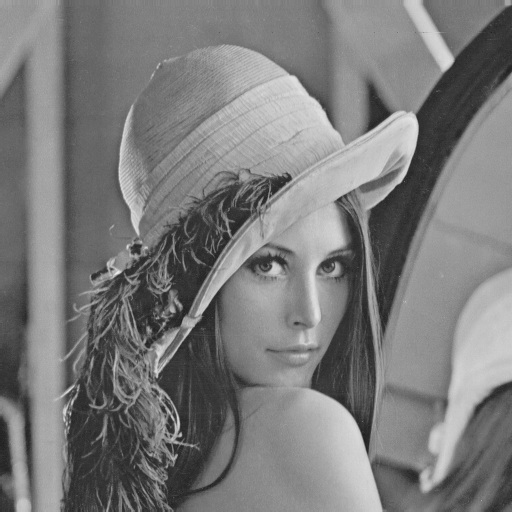
\includegraphics[keepaspectratio=true, scale=0.33]{images/lena.jpg}{}		
    }
    \hfill
    \subfloat[Magnitude representation\label{image-2:lena}]{
		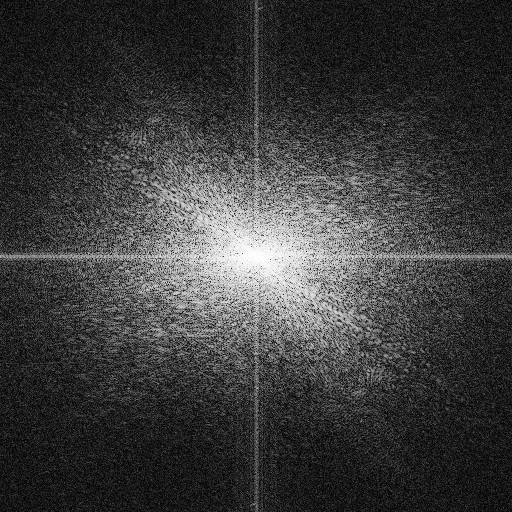
\includegraphics[keepaspectratio=true, scale=0.33]{images/lena_transformed.jpg}{}
    }
	\caption{Original image \ref{image-1:lena} transformed and represented with a quadrant shifted magnitude visualization (magnitude scale skewed for better visuals). \ref{image-2:lena}. }
    \label{fig:twodimentransform}
\end{figure}

The \gls{FFT} algorithm for two dimensional data, such as images, is first transformed row wise (each row as a separate sequence) and then a transform of each column. The implementation performs a row wise transformation and then transposes the whole image twice, see figure \ref{lst:cuda:host-2d-example}. A transformed image is shown in figure \ref{fig:twodimentransform}.

\begin{figure}[htbp]
	\centering
	\begin{framed}
		\includestandalone[width=\textwidth]{code/cuda-host-2d}	
	\end{framed}
	\caption{CUDA host code for the \gls{2D} \gls{FFT} algorithm.}
	\label{lst:cuda:host-2d-example}	
\end{figure}

The difference between the \gls{FFT} kernel for \gls{1D} and \gls{2D} are the indexing scheme. \gls{2D} are indexed as rows at \code{blockIdx.x} and columns at $\code{threadIdx.x} + \code{blockIdx.y} \cdot \code{blockDim.x}$. For \gls{2D} \code{blockIdx.z} is used as the sequence id in a batch.

\subsubsection{Transpose}

The transpose kernel uses a different index mapping of the 2D-data and blocks/threads then the \gls{FFT} kernel. The data is tiled in a grid pattern where each tile represents one block, indexed by \code{blockIdx.x} and \code{blockIdx.y}. The tile size is a multiple of 32 for both dimensions and limited to the size of the shared memory buffer, see table \ref{tab:threads-per-block} for specific size per technology. To avoid banking issues, the last dimension is increased with one but not used. However, resolving the banking issue have little effect on total running-time so when shared memory is limited to 32768, the extra column is not used. The tiles rows and columns are diveded over the \code{threadIdx.x} and \code{threadIdx.y} index respectively. See figure \ref{lst:cuda:device-transpose} for code example.

Shared memory example: The {\CU} shared memory can allocate 49152 bytes and a single data point require $\code{sizeof(float)} \cdot 2 = 8$ bytes. That leaves room for a tile size of $64 \cdot (64 + 1) \cdot 8 = 33280$ bytes.

\begin{figure}[H]
	\centering
	\begin{framed}
		\includestandalone[width=\textwidth]{code/cuda-device-transpose}	
	\end{framed}
	\caption{CUDA device code for the transpose kernel.}
	\label{lst:cuda:device-transpose}	
\end{figure}

The transpose kernel uses the shared memory and tiling of the image to avoid large strides through global memory. Each block represents a tile in the image. The first step is to write the complete tile to shared memory and synchronize the threads before writing to the output buffer. Both reading from the input memory and writing to the output memory is performed in close stride. Figure \ref{fig:transpose-memory} shows how the transpose is performed in memory.

\begin{figure}[H]
	\centering
	\includestandalone[width=\textwidth]{figures/transpose-tile}
	\caption{Illustration of how shared memory is used in transposing an image. Input data is tiled and each tile is written to shared memory and transposed before written to the output memory. }
	\label{fig:transpose-memory}
\end{figure}

\subsection{Differences}%
\subsubsection{Setup}%
The majority of differences in the implementations was related to the setup phase. The {\CU} implementation is the most straight forward, \code{cudaMalloc(...)} to allocate a buffer and \code{cudaMemcpy(...)} to populate it. With {\CU} you can write the device code in the same file as the host code and share functions. {\OCL} and {\GL} require a \code{char *} buffer and is most practical if written in seperate file and read as a file stream to a \code{char} buffer. {\DX} Shaders are most easily compiled from file. Figure \ref{fig:code:setup} demonstrates a simplified overview of how to setup the kernels in the different technologies.

\begin{figure}
	\centering
	\def \setupWidth {\textwidth / 2 - 20pt}	
	\subfloat[{\OCL} setup\label{setup:cu}]{		
		\fbox{\includestandalone[width=\setupWidth]{code/setup/cu}}
	}	
	\hfill
	\subfloat[{\OCL} setup\label{setup:ocl}]{		
		\fbox{\includestandalone[width=\setupWidth]{code/setup/ocl}}
	}
	\newline
	\subfloat[{\DX} setup\label{setup:dx}]{		
		\fbox{\includestandalone[width=\setupWidth]{code/setup/dx}}
	}
	\hfill
	\subfloat[{\GL} setup\label{setup:gl}]{		
		\fbox{\includestandalone[width=\setupWidth]{code/setup/gl}}
	}
	\caption{A overview of the setup functions for a kernel launch and buffer initialization.}
	\label{fig:code:setup}
\end{figure}

\subsubsection{Kernel execution}

Kernel execution in {\CU} is very much like any C-like language and the only difference is that the kernel launch syntax, $<<<$ and $>>>$, setting number of blocks and threads.

The other technologies require some more setup, {\OCL} and {\GL} set one parameter per line. {\OCL} maps with index whereas {\GL} maps with a string to the parameter. {\DX} is best suited to use a constant buffer for the parameters, the constant buffer is read only and accessible globally over the kernel. {\DX} and {\GL} share a similar launch style where the compute shader is set as the current program and then a dispatch call is made with the group (block) configuration. See table \ref{tab:kernel-execution} for a list of how the kernels are launched.

\begin{table}[H]
	\centering
	\includestandalone[width=\textwidth]{tables/kernel-execution}
	\caption{Table illustrating how to set parameters and launch a kernel.}
	\label{tab:kernel-execution}
\end{table}

\subsubsection{Kernel code}

This is the part where the code differ the least on but a few points. {\CU} have the strongest support for a {\CPP} -like language and only adds a function type specifier. The kernel program is accessible from the host via the \code{\_\_global\_\_} specifier. {\OCL} share much of this but restricted to a C99-style in the current version (2.0). One difference is how one can reference global and local buffers, these must be specified with the specifier \code{\_\_global} or \code{\_\_local}.

{\DX} and {\GL} Compute Shader is coded in \gls{HLSL} and \gls{GLSL} respectively. These languages are similar and share the same level of restrictions compared to CUDA C/C++ and {\OCL} C-code. Device functions can not use pointers or recursion. However these are of little importance for the performance since all code is in-lined in the compilation/building of the kernel program.

\subsubsection{Synchronization}

The synchronization of threads and blocks is slightly different, CUDA have the options to synchronize threads within a block and to synchronize host and device, the equivalent exists in all but {\DX} (DirectX 11) where the device synchronization is not done trivially as with a blocking function call. See table \ref{tab:kernel-synchronization} for the code used for each technology.

\begin{table}[H]
	\centering
	\includestandalone[width=\textwidth]{tables/kernel-synchronization}
	\caption{Synchronize functions regarding within blocks/groups and between host and device. CUDA, {\OCL} and {\DX} uses the same kernel stream to run them sequentially; {\GL} uses the command \code{glMemoryBarrier(GL\_SHADER\_STORAGE\_BARRIER\_BIT)} to ensure kernels are run in the same order as launched.}
	\label{tab:kernel-synchronization}
\end{table}

\section{Benchmark application CPU}

\subsection{FFT with OpenMP}

The {\OMP} implementation benefits in performance from calculating the twiddle factors in advance. The calculated values are stored in a buffer accessible from all threads. The next step is to calculate each stage of the \gls{FFT} algorithm. Last is the output index calculation where elements are reordered. See figure \ref{fig:omp:overview} for an overview.

\begin{figure}
	\centering
	\includestandalone[width=\textwidth]{figures/omp-overview}
	\caption{OpenMP implementation overview transforming sequence of size $N$.}
	\label{fig:omp:overview}
\end{figure}

\subsubsection{Twiddle factors}

The twiddle factor are stored for each butterfly operation. To save time, only the real part are calculated and the imaginary part is retrieved from the real parts due to the fact that $\sin(x) = \cos(\pi/2 + x)$ and $\sin(\pi/2 + x) = -\cos(x)$ to store. See figure \ref{tab:omp:twiddle-overview} for an example. The calculations will be split among the threads by static scheduling in two steps, first calculate the real values, secondly copy from real to imaginary.

\begin{table}[H]
	\centering
	\begin{tabular}{|l|l|r|}
	\multicolumn{3}{c}{Table $W$} \\ \hline
	$i$ & $\Re(W)$ & $\Im(W)$ \\ \hline
	0 & $\cos(\alpha \cdot 0)$ & $\Re(W[4])$ \\
	1 & $\cos(\alpha \cdot 1)$ & $\Re(W[5])$ \\
	2 & $\cos(\alpha \cdot 2)$ & $\Re(W[6])$ \\
	3 & $\cos(\alpha \cdot 3)$ & $\Re(W[7])$ \\	
	4 & $\cos(\alpha \cdot 4)$ & $-\Re(W[0])$ \\
	5 & $\cos(\alpha \cdot 5)$ & $-\Re(W[1])$ \\
	6 & $\cos(\alpha \cdot 6)$ & $-\Re(W[2])$ \\
	7 & $\cos(\alpha \cdot 7)$ & $-\Re(W[3])$ \\ \hline
\end{tabular}
	\caption{Twiddle factors for a 16-point sequence where $\alpha = (2 \cdot \pi) / 16$. Each row $i$ corresponds to the $i$th butterfly operation.}
	\label{tab:omp:twiddle-overview}
\end{table}

\subsubsection{Butterfly}

The same butterfly operation uses the constant geometry index scheme. The indexes are not stored from one stage to the next but it makes the output come in continues order. The butterfly operations are split among the threads by static scheduling.

\subsubsection{Bit Reversed Order}

See figure \ref{fig:omp:bit-reverse-order} for code showing the bit reverse ordering operation in C/C++ code.

\begin{figure}[H]
	\centering
	\begin{framed}
		\includestandalone[width=\textwidth]{code/omp-bit-reverse}	
	\end{framed}
	\caption{ C/C++ code performing the bit reverse ordering of a N-point sequence. }
	\label{fig:omp:bit-reverse-order}
\end{figure}

\subsection{FFT 2D with OpenMP}

The implementation of \gls{2D} \gls{FFT} with {\OMP} run the transformations row wise and transposes the image and repeat. The twiddle factors are calculated once and stays the same.

\subsection{Differences with GPU}

The OpenMP implementation differs from the \gls{GPU} with the fact that twiddle factors are pre computed and it uses the constant geometry implementation in all stages. The amount of parallel threads are on the {\INTELCPU} four whereas on the \gls{GPU} in the order of up to 192 (seven warps, one per \gls{SM}, with 32 threads each). This highly effects performance when the size of the problem grows.

\section{Benchmark configurations}

\subsection{Limitations}

All implementations are limited to handle sequences of $2^n$ length or $2^m \times 2^m$ where $n$ and $m$ are integers with maximal value of $n = m + m = 26$. The selected \gls{GPU}s have a maximum of 2GB global memory available. The limitation is required since the implementation uses a total of $2^{26} \cdot \code{sizeof(float2)} \cdot 2 = 1073741824$ bytes. However on the {\AMDCARD} card, problems with {\DX} and {\GL} set the limit lower. {\DX} handled sizes of $n <= 2^{24}$ and {\GL} $n <= 2^{24}$ and $m <= 2^{9}$.

\subsection{Testing}

All tests executed on the \gls{GPU} utilize some implementation of event time stamps. The time stamp event retrieve the actual start of the kernel if the current stream is busy. The \gls{CPU} implementations used Windows \emph{QueryPerformanceCounter} function, which is a high resolution ($<1{\micro}s$) time stamp.

\subsection{Reference libraries}

A reference libraries per platform was included to compare how well the FFT implementation performed. The \emph{\FFTW} library for the \gls{CPU}, runs a planning scheme to create an execution plan for each environment and data input size. Similar strategy is used in the {\CUFFT} and {\CLFFT} libraries used for the {\NVCARD} and {\AMDCARD} respectively. Table \ref{tab:external-implementations} sums up information about the external libraries.

\begin{table}
	\centering
	\begin{tabular}{|l|l|l|l|}
	\hline
	Platform & Model & Library name & Version \\ \hline
	NVIDIA GPU & GeForce GTX 670 & cuFFT & TODO \\
	AMD GPU & Radeon R7 260X & clFFT & 2.8.0 \\ \hline
	Intel CPU & Core i7 3770K 3.5GHz & FFTW & 3.3.4 \\ \hline
\end{tabular}
	\caption{Libraries included to compare with the implementation.}
	\label{tab:external-implementations}
\end{table}
%\chapter{Results}\label{cha:Results}



\chapter{Discussion and conclusions}

\todo{Do discussion, conclusions and future work here}


\part*{Appendix}
\appendix
%\chapter{Trista saker}\label{cha:boring}
Långa beräkningar brukar bli rätt trista\dots

Detta är ett appendix-kapitel.  Jämför med appendixet i \chapterref{cha:Research}.

\section{Bädda sängen}

Den här beräkingen är så trista att vi kallar den \emph{att bädda sängen}.

\section{Diska}

Den här beräkingen är så trista att vi kallar den \emph{att diska}.

%\chapter{\rtthesis documentation and \LaTeX{} tips}\label{cha:rtthesis}

This document is not only an example that you can use to get started with the \rtthesis class, it also contains written instructions for how to use the class, and some general tips on how to use \LaTeX{} to produce a beautiful thesis.  As we do so in this chapter, we also get the opportunity to look at some theorem-like environments, which you can alter the look of by changing the options given to the \rtthesis class.

\section{Basic setup}\label{sec:basic-setup}
%
You must decide on an input encoding from start, and select the corresponding class option from \tableref{tab:inputenc} on \pagepageref{tab:inputenc}.  You must also tell \rtthesis whether you intend to use part sectioning or not, see \tableref{tab:part-options}.  There are many more class options, but they will be mentioned below where there is room for a more detailed discussion for the corresponding features.

Information about the thesis, which is needed to produce the thesis itself as well as the thesis cover and the “spikblad”, is passed to \rtthesis using the command \texcommand{setupThesis}.  The command is called in the following way, where the most common key-value pairs are listed in \tableref{tab:setupThesis} (the remaining key-value pairs concern master's theses, see \sectionref{sec:msc})):

\begin{minipage}{1.0\linewidth}
  \verbatimsize
\begin{verbatim}
\setupThesis{
  key1=value1,
  key2=value2,
  ...
}
\end{verbatim}
\end{minipage}

If a PhD thesis has an interesting illustration on the cover, it is customary to provide a caption for the illustration.  The caption will be printed on the back of the title page, and is set up by redefining the command \texcommand{rtcoverinfo}.  For instance, it may look like this:

\begin{minipage}{1.0\linewidth}
  \verbatimsize
\begin{verbatim}
\renewcommand{\rtcoverinfo}{\textbf{Cover illustration:}  Block
diagram showing the structure of the control scheme proposed in
\chapterref{cha:cool-control}}
\end{verbatim}
\end{minipage}


\begin{table}[tbp]
  \centering
  \caption{\label{tab:part-options}%
    Class options that inform \rtthesis whether part sectioning will be used or not.}

  \begin{tabular}{l p{0.5\linewidth}}
    \toprule%
    \textbf{Class option} & \textbf{Meaning} \\
    \otoprule%
    \classoption{parts} & Prepare for \texcommand{part} as the topmost sectioning command.\\
    \classoption{noparts} & Prepare for \texcommand{chapter} as the topmost sectioning command.\\
    \bottomrule%
  \end{tabular}
\end{table}

\begin{table}[tbp]
  \centering
  \caption{\label{tab:setupThesis}%
    Key-value pairs recognized by \texcommand{setupThesis}.  Note that values that include white space are surrounded by braces.}

  \begin{tabular}{>{\ttfamily}r !{\texttt{=}} >{\ttfamily}l p{0.5\linewidth}}
    \toprule%
    \textbf{Key} & \textbf{Example value} & \textbf{Comment} \\
    \otoprule%
    author & \{My Name\} & \\
    title & \{Thesis title\} & \\
    subtitle & \{Good stuff\} & Optional. \\
    city & Norrköping & Default: \emph{Linköping} \\
    year & 2010 & \\
    isbn & isbn-isbn-isbn-isbn & \\
    type & phd & Must be either \emph{phd}, \emph{lic}, or \emph{msc}. \\
    thesisNo & 9999 & Number in series (the series is determined by the choice of thesis type). \\
    localID & 11 & Only used for licentiate's theses.  It is the last part of the local identifier \emph{\mbox{LIU-TEK-LIC-2010:11}} in this case.\\
    username & isyusername & Used to generate the author's email address. \\
    dedication & \{To my parents!\} & \\
    \bottomrule%
  \end{tabular}
\end{table}

\section{Page layout and related options}\label{sec:page-layout}
%
Theses are restricted to the S5 paper size.  How the S5 page is organized is up to you, but \rtthesis only allows you to choose from two predefined layouts, and only one of them is recommended.  To get your own layout you should make a copy of \textfilename{rtthesis.cls} and modify the code for one of the existing class options for layout.  The class options for page layout are given in \tableref{tab:page-layout}.

At the time of writing, the printers used by LiU-Tryck print on A4 paper (physical size), which is then cropped to S5 (logical size).  Similarly, when you print draft versions of your thesis on your office printer, it is very likely that the used physical paper size will be A4.  Hence, it makes sense to let \rtthesis control how the S5 logical page is placed on the A4 physical paper.  In this case, \rtthesis will produce a \textsc{pdf} with pages in the A4 format, with content restricted to the S5 format.  On the other hand, when you produce a \textsc{pdf} that is meant to be read on a computer screen, the page size should be exactly S5.  When targeting the A4 physical format, it is possible to get crop marks for the S5 box, and to put some information about each page outside the S5 box.  The related class options are given in \tableref{tab:page-layout}.

To ensure that you really get the page layout you think when you send your thesis file to the printer's, the best option \emph{should} be to use the \classoption{crop} option.  However, they will tell you differently, since they think it's \emph{their} job to position the logical page on A4 and add crop marks.  Unfortunately, there is a lot of manual work in the process, so there is a (substantial?!) risk that the content of your pages will be shifted with respect to the S5 box of your layout\ldots

\begin{table}[tbp]
  \centering
  \caption{\label{tab:page-layout}%
    Class options related to page layout.  The most important one to remember is \classoption{crop} (since  \classoption{S5} and \classoption{pdf} are default).}

  \begin{tabular}{l p{0.5\linewidth}}
    \toprule%
    \textbf{Class option} & \textbf{Meaning} \\
    \otoprule%
    \classoption{S5} & Recommended layout.  Margin paragraphs are tiny (see \sectionref{sec:research:history} for examples), and should only be used for comments that will be removed in the final version of the thesis.  Default.\\
    \classoption{S5MP} & Layout to use if you are serious about margin paragraphs.  Not recommended, since the S5 format is too narrow to really fit margin paragraphs of reasonable width. \\
    \classoption{nailing} & Layout for the “spikblad”.  Not for theses! \\
    \midrule%
    \classoption{pdf} & Produce pages in the S5 format.  Default.\\
    \classoption{onA4} & Logical S5 page on a \textsc{pdf} page of size A4.\\
    \classoption{info} & Write information about each page above the logical S5 page.\\
    \classoption{crop} & Same as \classoption{onA4} with \classoption{info} and crop marks.\\
    \classoption{noInfo} & Turn off the effect of \classoption{info}.\\
    \classoption{draft} & Same as \classoption{onA4}, but pictures are blank and overfull \texttt{hbox}es stand out.\\
    \bottomrule%
  \end{tabular}
\end{table}

Although only weakly related to page layout, this section ends with a tip for how to change the size of the chapter numbers (some users find them much too big).  The font is controlled using the \styname{sectsty} package, and it follows that it can be redefined by, for instance,

\begin{minipage}{1.0\linewidth}
  \verbatimsize
\begin{verbatim}
\chapternumberfont{\fontsize{60mm}{63mm}\selectfont}
\end{verbatim}
\end{minipage}

\section{Front-matter environments}

There are environments defined for typical sections in the front-matter\footnote{The \emph{front-matter} is everything that goes in the beginning of the thesis, before the page numbered~\emph{1}.}.  The most important purpose of providing these environments is that they take care of the table of contents and the \textsc{pdf} bookmarks for you.  The environments are \envname{abstract}, \envname{preface}, \envname{acknowledgments}, and \envname{notation}.

The environment \envname{abstract} accepts the language used inside the environment as an optional argument (which defaults to \texttt{english}).  If the language is set to \texttt{swedish}, the title of the abstract will be \emph{Populärvetenskaplig sammanfattning}, in accordance with the Linköping University requirements on theses written in English.

Inside the \envname{notation} environment, you can put anything you like, and maybe the \envname{notationtabular} environment provided by \rtthesis suits your needs.  In order to define this environment, \rtthesis loads the two packages \styname{array} and \styname{ctable}, and also defines the command \texcommand{otoprule} to mean the same as \texcommand{toprule}.  See \tableref{tab:notationtabular} regarding how to change the look of \envname{notationtabular}.

\begin{table}[tbp]
  \centering
  \caption{\label{tab:notationtabular}%
    Legal option values to the \envname{notation} environment.  The options control the look of the \envname{notationtabular} environments used inside the \envname{notation} environment.  The initial definition of \envname{notationtabular} is the same as that obtained by passing the option \classoption{new}.}

  \begin{tabular}{l p{0.5\linewidth}}
    \toprule%
    \textbf{Option} & \textbf{Meaning} \\
    \otoprule%
    \emph{emty} & Do not redefine \envname{notationtabular}.  Default.\\
    \classoption{old} & Make \envname{notationtabular} produce a plain \LaTeX{} table with double horizontal lines under the table headings, and a vertical line separating the two columns.\\
    \classoption{new} & Make \envname{notationtabular} produce a table according to the guidelines in \citet{Mori07Tables} using the \styname{ctable} package.\\
    \bottomrule%
  \end{tabular}
\end{table}

There is a class option called \classoption{noextras}, which was intended to inhibit the effect of the \texcommand{maketitle} command, and redefine the front-matter environments to not produce any output.  However, the option is not working well at the moment.  On the other hand, as the time it takes to compile a thesis on a modern computer is very short, it is rather unclear why someone would like to use this feature anyway.


\section{Abbreviations}

Automatic control is a \LaTeX{}-friendly community.  This means that everything you produce is expected to look good.  We begin with a basic result.

\begin{theorem}\label{th:abbr-in-sc}
  Abbreviations, such as \abbrARMA, look best in small caps.

  \begin{proof}
    Just compare with “ARMA”.
  \end{proof}
\end{theorem}

However, it is important that the small caps match the sorrounding text, compare the statement in the theorem above with the following variation of it, in italics instead of slanted text:
\begin{quotation}
  \noindent\textit{Abbreviations, such as \abbrARMA\footnote{This will cause a \LaTeX{} warning.} or {\normalfont\textsc{arma}}, will stick out in a terrible way if you don't watch out!}
\end{quotation}
This is why the \rtthesis class uses slanted text rather than italics in theorems rather when slanted small caps are available.

Unfortunately, \rtthesis does currently not provide a way to make small caps look good in italics, which leads to the following corollary to \theoremref{th:abbr-in-sc}.

\begin{corollary}
  One has to make a choice between
  \begin{itemize}
  \item Beautiful abbreviations using small caps (instead of ordinary upper case).
  \item Pretty text typeset in italics (instead of slanted text).
  \end{itemize}
\end{corollary}

\section{Definitions}

Let us discuss another theorem-like environment while we have some examples of similar environments to compare with in the previous section.  That is, let us discuss the \envname{definition} environment (and the similar environments \envname{assumption} and \envname{remark}).  All the theorem-like environments are defined in a separate package, \styname{rtthesis-theorems}, so that they can be used with other document classes as well.  The definition below is an example of a definition with a title.

\begin{definition}[Definition]
  A \emph{definition} is a precise explanation of the meaning of a word or concept.  It may be tempting to include examples in a definition, but a good definition should not depend on examples as part of the definition.  However, examples are often useful to clarify a definition, and should appear near the definition.

  A short definition may require just a single paragraph, while a more complex definition may require a few paragraphs.  Some definitions will also make use of displayed math.
\end{definition}

One problem one has to consider if definitions are not restricted to just one paragraph, is how to show the reader where the definition ends.  In theorems, it is common to use italics or slanted text (for brevity, we will not mention italics from here on) to show where the theorem statement ends, but for definitions it may be desirable to use the slanted text to emphasize the word or concept being defined.  (It is arguably more clear to highlight the new word or concept using slanted text with upright surrounding text, than vice versa.)  To use an upright font for the definitions may also be a way of avoiding to heavy use of slanted text.

Various options related to the appearance of theorem-like things (in \LaTeX{}, a definition is a kind of theorem) are described in \tableref{tab:theorems}.  \Tableref{tab:definitions} (used also to illustrate tables) contains some suggestions regarding combinations of options for the \envname{definition} environment and options for paragraph breaks.

\begin{table}[tbp]
  \centering
  \caption{\label{tab:theorems}%
    Class options related appearance of theorem-like environments.  The \emph{theorem-like environments} defined by \rtthesis are \envname{theorem}, \envname{proposition}, \envname{lemma}, \envname{corollary}, \envname{definition}, \envname{assumption}, and \envname{remark}.  The \emph{definition-like environments} are a subset of the \emph{theorem-like environments}, consisting of the environments \envname{definition}, \envname{assumption}, and \envname{remark}. See also \tableref{tab:fonts} regarding the fonts used in theorems.}

  \begin{tabular}{l p{0.5\linewidth}}
    \toprule%
    \textbf{Class option} & \textbf{Meaning} \\
    \otoprule%
    \classoption{break} & Put line breaks after the titles of the environments \envname{theorem}, \envname{proposition}, \envname{lemma}, and \envname{corollary}.\\
    \classoption{nobreak} & Never put line breaks after titles of theorem-like environments.  Default.\\
    \midrule%
    \classoption{definition=naked} & Definition-like environments look like the surrounding text, and are only isolated by some vertical white space.  Default.\\
    \classoption{definition=theorem} & Definition-like environments use same font as the \envname{theorem} environment, and are isolated by some vertical white space.\\
    \classoption{definition=marks} & Definition-like environments look like the surrounding text, and are isolated by small marks.  Strongly recommended if \classoption{parskip} is used.\\
    \midrule%
    \classoption{nosharecounter} & Use separate numbering sequences for each theorem-like environment and the \envname{example} environment.\\
    \classoption{sharecounter} & Use one numbering sequence for theorem-like environments, and the \envname{example} environment.\\
    \bottomrule%
  \end{tabular}
\end{table}

Sometimes, a definition may be given without a title.  The next definition is an example of this, even though it is questionable whether it was a good idea to omit the title in this particular case.

\begin{definition}
  An \emph{environment} in \LaTeX{} is a construct that is entered with the command \texcommand{begin\{\ldots\}} and exited with the command \texcommand{end\{\ldots\}}, where “\ldots” should be the name of the environment.
\end{definition}

In \tableref{tab:theorems}, there are three options related particularly to how \envname{definition}, \envname{assumption}, and \envname{remark} are typeset.
\begin{itemize}
\item With \classoption{definition=naked} (default) the definitions are typeset in upright font, and there is nothing on the page that marks the end of the definition.
\item With \classoption{definition=theorem} the definitions are typeset in the same style as theorems.  Since theorems are supposed to be typeset in slanted text, this will make it clear where the definition ends.
\item With \classoption{definition=marks} the beginning and end of definitions will be indicated with small marks.  Compare how the end of a proof is marked with a square box!  The current implementation has some problems with placing the marks if the definition ends with a displayed equation, but this can be compensated for by manual insertion of a \texcommand{vspace} command.
\end{itemize}

You may judge from the following example whether manual insertion of a \texcommand{vspace} command is necessary to make the definition ending with a displayed equation look alright.

\begin{definition}
  The factorial (denoted by the postfix operator $!$), defined for natural numbers, is given by
  \begin{equation*}
    n! =
    \begin{cases}
      1, & \text{if $n = 0$} \\
      n \cdot (n-1) \cdot \dotsc \cdot 1, & \text{otherwise}
    \end{cases}
  \end{equation*}
\end{definition}

This paragraph only serves to highlight the vertical white space below the definition ending with a displayed equation.  Note that one way to avoid problems with this kind of definitions is to rewrite them so that they don't end with displayed equations.

All definitions in this section have been entered as isolated paragraphs; that is, there is an empty line in the source code of the document before and after each \envname{definition} environment.  Although not recommended, \rtthesis supports definitions that are connected with the preceding paragraph, in which case the usual vertical space (if any) between paragraphs will not be inserted.  \emph{Be careful so that you don't omit the paragraph breaks by mistakes, since it makes a difference that may be hard for proofreaders to spot!}  As an example of a definition written in the same paragraph as the preceding text,
\begin{definition}
  A \emph{paragraph} (according to Oxford American Dictionaries) is a distinct section of a piece of writing, usually dealing with a single theme and indicated by a new line, indentation, or numbering.
\end{definition}
There is no paragraph break in the source code between the definition above and this text, but currently this cannot be seen in the typeset document.  If you know how to solve this, let the \rtthesis maintainer know!  If you want to learn about the \TeX{} mechanisms involved, see \citet{RyckoJackowski93TeXIndentPar}.

\section{Theorem titles}
%
The class lets you control the white space that separates a theorem title from the theorem statement.  The options appear in \tableref{tab:theorems}.  With the class option \classoption{break} (default), you will get a line break.  With \classoption{nobreak}, you will just get horizontal space.  Not all types of theorem-like environments will be affected by the \classoption{break} option, so to get things exactly they way you want, you may have to make your own modified copy of the \rtthesis class.  Try to recompile the document with the two different options and compare the result!

\section{To share or not to share counters}\label{sec:rtthesis:sharecounter}
%
Other things to think about regarding style include whether to use the same counter for all sorts of theorem-like things.  Again, the options appear in \tableref{tab:theorems}.  Some like to make the number of important theorems to stand out by having a separate counter (as in \citet{Khalil02NonlinearSystemsBook}), while other prefer to use as few counters as possible in order to make it easy to locate referenced items (as in \citet{Rugh96LinearSystemsBook}).  The two alternatives are supported in \rtthesis, via the options \classoption{sharecounter} and \classoption{nosharecounter}.

\section{Completely customized theorem-like environments}\label{sec:rtthesis:custom-theorems}
%
If you don't like the way \rtthesis sets up theorem-like environments (listed in the caption of \tableref{tab:theorems}) for you, you may pass the class option \classoption{notheorems}.  Then \styname{amsthm} will not be loaded, none of the theorem-like environments will be defined, and it is up to you to define your own environments.  If you decide to do so, using the \styname{amsthm} package will be a good idea.

\section{The \envname{example} environment}
%
The \envname{example} environment defined by the \rtthesis class is \emph{not} a floating environment, but is simply used to highlight that the text inside the environment is just an example of something more general that you have explained before.  Just as with the theorem-like environments, the environment is defined in a separate package, \styname{rtthesis-example}, so that it can be used with other document classes as well.

\begin{example}
  As an example of the \envname{example} environment, we include a little example here.  You can use this example to see how the options described in \sectionref{sec:rtthesis:sharecounter} affects the numbering of the environment.

  Depending on where this example ends up in the typeset document, you may also have the chance to see the ugly stretched vertical space that sometimes appears at the top and bottom of the environment.
\end{example}

There are three lengths you may play with the fine tune the appearance of examples, explained in \tableref{tab:example-lengths}.  Clearly, it would be possible to introduce additional parameters, but currently the corresponding aspects of the environment are hard-coded into \rtthesis.

\begin{table}[tb]
  \centering
  \caption{\label{tab:example-lengths}%
  The lengths used to control the appearance of the \envname{example} environment.  Note that the environment tries to compensate for the current value of \texcommand{parskip}, so you may not always get exactly what you'd expect.  Also, the meaning of the distance between the upper stroke and the text is somewhat arbitrary in order to allocate space for the example title.}

  \begin{tabular}{>{\small\ttfamily}l p{0.1\textwidth} p{0.4\textwidth}}
    \toprule
    {\normalsize\normalfont\textbf{Length}} & \textbf{Default} & \textbf{Purpose} \\
    \otoprule
    $\backslash$exampleLineWidth & $\unit{0.6}{pt}$ & Thickness of the strokes. \\
    \midrule
    $\backslash$exampleTopBotInnerMargin & $\unit{2}{ex}$ & Vertical space between strokes and contents of the example. \\
    \midrule
    $\backslash$exampleTopBotOuterMargin & $\unit{1}{em}$ \texttt{plus} $\unit{1}{ex}$ \texttt{minus} $\unit{1}{ex}$ & Vertical space surrounding the example. \\
    \bottomrule
  \end{tabular}
\end{table}

As is mentioned in the example above, there is sometimes problem with vertical space at the top and bottom of the \envname{example} environment.  During the page breaking process (see \sectionref{sec:tipt:page-breaking}) you could consider to add something like
{\verbatimsize
\begin{verbatim}
  \vspace{-1\baselineskip}
\end{verbatim}}
to reduce such artifacts.  Even better, if you know how to correct this in the definition of the environment, let the \rtthesis maintainer know!  The paper \citet{RyckoJackowski93TeXIndentPar} is recommended for anyone interested in the lesser known details of \TeX{} that one has to grasp in order to really solve the problem.

\section{Captions}\label{sec:rtthesis:captions}
%
The \rtthesis class loads the \styname{captions} package to obtain good-looking captions.  Captions are set up assuming that table captions will be placed above the table they belong to.  Many authors find this confusing since figure captions are always placed below the figure they belong to.  If you want to put table captions below the table you need to adjust the spacing around the caption by putting the following line in your personal style file:
{\verbatimsize
\begin{verbatim}
\captionsetup[table]{position=bottom}
\end{verbatim}}

Note that the command above only changes the spacing around the caption.  You still have to put the code for each caption relative to the tabular itself consistently with the captions setup.  Two tables are included in this document for illustration.  \Tableref{tab:definitions} indicates the many combinations of options that the \envname{definition} environment has been designed to work with.  The next one, \tableref{tab:chapters} is just a stupid table telling where the different chapters in this document begin.  For comparison, a typical automatic control block diagram has been included in \figureref{fig:feedback}.

Some nice guidelines for table creation in \LaTeX{} are given in \citet{Mori07Tables} (it is just two clicks away!).

\begin{table}[p]
  \centering
  \caption{\label{tab:chapters}%
    Different combinations of class options that affects the \envname{definition} environment.  The code for this caption appears at the beginning of the \envname{table} environment.  It would have had the desired distance to the tabular if the default caption setup of \rtthesis was used, but this document has been set up for table captions below the corresponding tabular.}
  \begin{tabular}{c l c}
    \toprule%
    \textbf{Chapter} & \textbf{Title} & \textbf{Page} \\
    \otoprule%
    \ref*{cha:intro} & \nameref{cha:intro} & \pageref{cha:intro} \\
    \ref*{cha:Research} & \nameref{cha:Research} & \pageref{cha:Research} \\
    \ref*{cha:rtthesis} & \nameref{cha:rtthesis} & \pageref{cha:rtthesis} \\
    \ref*{cha:boring} & \nameref{cha:boring} & \pageref{cha:boring} \\
    \bottomrule%
  \end{tabular}
\end{table}

\begin{table}[p]
  \centering
  \caption{\label{tab:definitions}%
    Different combinations of class options that affects the \envname{definition} environment.  The code for this caption appears at the end of the \envname{table} environment.  It will be too close to the tabular using the default settings of \rtthesis (but note that this document has been setup differently, see \sectionref{sec:rtthesis:captions}).}

  \begin{tabular}{>{\bfseries}l c c c}
    \toprule%
    & \multicolumn{3}{c}{\bfseries\texttt{definition=}} \\
    & \bfseries\classoption{naked} & \bfseries\classoption{theorem} & \bfseries\classoption{marks} \\
    \otoprule%
    \classoption{noparskip} & OK & Avoid & OK \\
    \midrule
    \classoption{parskip} & Bad & Avoid & OK \\
    \bottomrule%
  \end{tabular}
\end{table}

\begin{figure}[p]
  \centering
  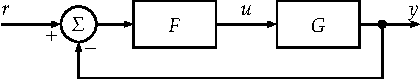
\includegraphics{feedback}
  \caption{\label{fig:feedback}%
    A simple illustration in a floating \envname{figure} environment.  Note that figure captions are always placed under the corresponding figure, and hence that the caption code should always appear at the end of the \envname{figure} environment.}
\end{figure}

\section{Hyperlinks}
%
For readers our the electronically published version of your thesis, as well as yourself while your are working on it, it is very convenient to have working hyperlinks in the document.

\subsection{Basic setup}
%
Basically, hyperlinks are obtained by using the \styname{hypreref} package. However, this package has quite a lot of compatibility issues with other packages, and knowledge about how to deal with these issues is coded into the \rtthesis class.  That is, all you should have to do to get hyperlinks in your document is to specify the \classoption{hyperref} option to \rtthesis.  The class options related to the linking infrastructure of the document are listed in \tableref{tab:hyperref}.

At the time of writing \rtthesis does not call \texcommand{hypersetup} with information about document title, keywords, and other information provided to \texcommand{setupThesis} (see \tableref{tab:setupThesis}).  If someone wants this, it shouldn't be hard to do.

\begin{table}[tbp]
  \centering
  \caption{\label{tab:hyperref}%
    Class options related to (hyper) linking infrastructure.}

  \begin{tabular}{l p{0.5\linewidth}}
    \toprule%
    \textbf{Class option} & \textbf{Meaning} \\
    \otoprule%
    \classoption{hyperref} & Turn on hyperlinks using the \styname{hyperref} package.  Default. \\
    \classoption{nohyperref} & Turn off hyperlinks, and compensate for commands no longer provided by the \styname{hyperref} package. \\
    \midrule%
    \classoption{backref} & Turn on bibliography back references.  Default. \\
    \classoption{nobackref} & Turn off bibliography back references.  (Currently required if you plan to use the features of \styname{bibunits}.)\\
    \bottomrule%
  \end{tabular}
\end{table}


\subsection{Hyperlinks and electronic publishing}
%
To make your dear hyperlinks survive all the way to the electronic publishing system, you may have to replace the file that is sent to e-press by LiU-tryck.  The problem is that LiU-tryck creates a compressed version of the file that is used in the printer, and the compression will remove nice features such as page numbers, hyperlinks, and bookmarks.  Fortunately, the guys at e-press seem to be understanding and will accept to publish a file that they receive directly from you.

\subsection{Page number formatting in the index}
%
If you use an index in your thesis, you will often want to change the formatting of certain page numbers in the index.  Without \styname{hyperref}, this could look like
{\verbatimsize
\begin{verbatim}
hyperlinks\index{hyperlinks|textit}
\end{verbatim}}
to get the page number for this occurrence of \emph{hyperlinks} to be typeset in italics.  The problem with this is that this page number will not be a hyperlink, while other page numbers will be hyperlinks to the correct page.  To get both italics and a hyperlink you need to define a special index formatting commands like the following.
{\verbatimsize
\begin{verbatim}
\newcommand{\hyperpageit}[1]{\textit{\hyperpage{#1}}}
\newcommand{\hyperpagebf}[1]{\textbf{\hyperpage{#1}}}
\newcommand{\hyperpagefootnote}[1]{\hyperpage{#1}n}
\end{verbatim}}

Now, you can write
{\verbatimsize
\begin{verbatim}
hyperlinks\index{hyperlinks|hyperpageit}
\end{verbatim}}
to get both italics and a hyperlink.  The \rtthesis class will provide a trivial definition of \texcommand{chapter} in case \styname{hyperref} is not loaded, so you may safely start to use the above definitions even if you are not sure whether you will use hyperlinks in the end.

\subsection{Friendlier hyperlinks}
%
The default mechanism for references in \LaTeX{}, being the command \texcommand{ref}, is modified as expected by the \styname{hyperref} package.  For instance, the number in “chapter~\ref{cha:rtthesis}” is linked to the beginning of the current chapter (if you click it, be sure to just the \emph{jump back} function of your \textsc{pdf} viewer to get back to here!).  However, all of “\hyperref[cha:rtthesis]{this}” is also a link to the same place.  That is, it is possible to other things than the number itself as links.  We could also make a reference that will never be linked, like in “chapter~\ref*{cha:rtthesis}”.

So, what's so friendly about this?  What I'm aiming at is that you can say “\hyperref[cha:rtthesis]{chapter~\ref*{cha:rtthesis}}”.  The code for this link is
{\verbatimsize
\begin{verbatim}
\hyperref[cha:rtthesis]{chapter~\ref*{cha:rtthesis}}
\end{verbatim}}

Of course, it is very annoying to repeat the key twice; first to point the hyperlink to the correct place, second to show the number of the chapter.  With the \texcommand{autoref} command from the \styname{hyperref} bundle, we get “\autoref{cha:rtthesis}”.  This is almost perfect.  The problem is that one cannot get an uppercase initial at the beginning of a sentence without redefining “chapter” to “Chapter“,
{\verbatimsize
\begin{verbatim}
\renewcommand{\Chaptername}{Chapter}
\end{verbatim}}
but then we will not get the nice lower case initial in the middle of a sentence.  Many authors don't bother about this and use uppercase initials irrespectively of where in a sentence the reference appears.

The only solution I (Henrik Tidefelt) knows of, is to define special commands for each type of reference.  A basic solution might look as follows.
{\verbatimsize
\begin{verbatim}
\newcommand{\chapterref}[1]{\hyperref[#1]{chapter~\ref*{#1}}}
\newcommand{\Chapterref}[1]{\hyperref[#1]{Chapter~\ref*{#1}}}
\end{verbatim}}

You should then use \texcommand{chapterref} in the middle of a sentence, and \texcommand{Chapterref} at the beginning of a sentence.  I you later decide that you want to have upper case initials everywhere, you just have to change your definitions to
{\verbatimsize
\begin{verbatim}
\newcommand{\chapterref}[1]{\hyperref[#1]{Chapter~\ref*{#1}}}
\newcommand{\Chapterref}[1]{\hyperref[#1]{Chapter~\ref*{#1}}}
\end{verbatim}}

A more complete solution will also provide commands for the plural forms “chapters” and “Chapters”.

It is also nice to use a similar technique for page references.  For instance, this chapter starts on \hyperref[cha:rtthesis]{page~\pageref*{cha:rtthesis}}, and such links can be created easily using a command like
{\verbatimsize
\begin{verbatim}
\newcommand{\pagepageref}[1]{\hyperref[#1]{page~\pageref*{#1}}}
\end{verbatim}}

Because of the many possible preferences for how to handle labels and references within documents, \rtthesis does not define any related commands.  The current section should give you some ideas of what can be achieved, and now it is up to you to design your own solution or borrow a solution from someone else (or simply stick with \texcommand{autoref} or the 1980's way of doing things)!

\section{Backreferences from the bibliography}
%
By default, \rtthesis uses the \styname{backref} package to put references from the bibliography back into the text.  The options for turning this feature on and off are listed in \tableref{tab:hyperref}.

By controlling this feature via the class, the choice whether to use it or not can be made orthogonal to the choice of whether to use \styname{hyperref} or not.

In addition to just loading \styname{backref}, \rtthesis will do a basic setup of the commands used to typeset the list of page numbers for each reference.  This behavior can easily be redefined without modifying the \rtthesis class file.  See the \styname{backref} documentation for details on how to do this!

\section{Using the \styname{bibentry} package}\label{sec:rtthesis:bibentry}
%
The \styname{bibentry} package makes it possible to use the information in the bibliography to present your publications at any place in the document.  In order to work independently of whether you use back references from the bibliography or not, you need to follow the pattern below each time you use the \texcommand{bibentry} command, where \texttt{KEY} is the same key to you publication that you would with use with any other citation command.

\begin{minipage}{1.0\linewidth}
  \verbatimsize
\begin{verbatim}
\begin{quotation}
  \nocite{KEY}\noindent
  \backrefparscanfalse\bibentry{KEY}.\backrefparscantrue
\end{quotation}
\end{verbatim}
\end{minipage}

To use the \envname{quotation} environment is just a suggestion — it will make the reference stand out by using a some what shorter text line width.  Note the period that follows the \texcommand{bibentry} command — the command leaves it up to you how to terminate the entry.  The \texcommand{nocite} command ensures that the reference appears in the bibliography, which is necessary to produce the entry.  The \texcommand{noindent} commands simply prevents the first line in the \envname{quotation} from being indented.  The commands \texcommand{backrefparscanfalse} and \texcommand{backrefparscantrue} are related to the \styname{backref} package used to produce back references from the bibliography, and should always surround the \texcommand{bibentry} command.  In case you have turned back references off using the \classoption{nobackref}, \rtthesis will provide substitutes for these two commands.


\section{Fonts}
%
Though basically not a task for a \LaTeX{} class, \rtthesis will assist in loading some font packages.  There are some class options that control this behavior, described below, and if these options are not good enough for you, you may have to make your own copy of the class and replace the font packages you don't like.  Options for font selection are listed in \tableref{tab:fonts}.

One reason, however, for letting \rtthesis handle the font selection is that this makes it possible for the class to do some things more intelligently.  At the moment, \rtthesis will help you make use of some of the goodies of KpFonts, if you choose to use that font.

\begin{table}[tbp]
  \centering
  \caption{\label{tab:fonts}%
    Class options related to fonts.  When slanted small caps are activated, theorem-like environments will use slanted text instead of italics.  The lower part of the table are examples of options that will be understood by the \styname{kpfonts} package, and are only meaningful in combination with the \classoption{kp} option.  (Note that options passed to \rtthesis, but that are not understood by \rtthesis will be passed on automatically by \LaTeX{} to loaded packages.)}

  \begin{tabular}{l p{0.5\linewidth}}
    \toprule%
    \textbf{Class option} & \textbf{Meaning} \\
    \otoprule%
    \classoption{kp} & Use KpFonts (Kepler) and activate slanted small caps.  Default.\\
    \classoption{times} & Use Times and deactivate slanted small caps.\\
    \classoption{lm} & Use Latin Modern and deactivate slanted small caps.\\
    \midrule%
    \classoption{largesmallcaps} & Let the small caps be slightly higher than an \emph{x}.  See the KpFonts documentation!\\
    \classoption{intlimits} & Placement of integration limits.  See the KpFonts documentation!\\
    \classoption{widermath} & Put just a little more horizontal space between entities in math mode.  See the KpFonts documentation!\\
    \bottomrule%
  \end{tabular}
\end{table}

\section{Hanging punctuation}
%
The \rtthesis class automatically loads the \styname{pdfcprot} package with its default settings.  It uses a pdf\TeX{} feature to make punctuation hang into the right margin.  If you don't like it, make your own copy of the class and comment out the line that loads the package.  One reason not to use it would be if your document will be (perhaps only occasionally) typeset using the old \TeX{} program, since this will lead to noticeable differences in the line breaks compared to when pdf\TeX{} is used.  No matter what you choose, make your choice \emph{before} you start working with the page breaks in your document!

\section{Paragraph breaks}
%
There are two common ways of visualizing paragraph breaks in a document, illustrated by the two examples below.  The look of paragraph breaks is controlled using the class options listed in \tableref{tab:parskip}.

\begin{table}[tbp]
  \centering
  \caption{\label{tab:parskip}%
    Class options related to formatting of paragraph breaks.}

  \begin{tabular}{l p{0.5\linewidth}}
    \toprule%
    \textbf{Class option} & \textbf{Meaning} \\
    \otoprule%
    \classoption{noparskip} & US style, see \exampleref{ex:paragraph-break-noparskip}.  Default.\\
    \classoption{parskip} & European style, see \exampleref{ex:paragraph-break-parskip}.\\
    \bottomrule%
  \end{tabular}
\end{table}

% \begin{example}[Default text]
%   This example does not mess with the lengths controlling the paragraph break format.  But you bet it ends in vmode!

% \end{example}

% It is good to see what it looks like if one puts text just below an example.

% \begin{example}[Default text]
%   This example does not mess with the lengths controlling the paragraph break format.  This one ends in hmode!
% \end{example}

\begin{example}[Indented first line]\label{ex:paragraph-break-noparskip}%
  \setlength{\parskip}{0pt}%
  \setlength{\parindent}{1.5em}%
  This style is still the most common.  It is particularly dominant in text written in the US.

  It is a matter of style whether to omit the indentation of the first line after a sectioning command such as \texcommand{chapter} or \texcommand{subsection}.  The omission is typically automated, but can also be enforced using the  \texcommand{noindent} command.

  One drawback of not having vertical space between paragraphs is that it will be harder for pdf\TeX{} to find good places for page breaks, compared to the option shown below.  If you like compact documents, however, this is the option for you!

  For testing purposes, this example ends with a paragraph break, so that \TeX{} is in \emph{vmode} at the end.  You should always avoid this, but the class will try to compensate for your mistakes\ldots

\end{example}

\begin{example}[Vertical white space]\label{ex:paragraph-break-parskip}%
  \setlength{\parskip}{1ex}%
  \setlength{\parindent}{0pt}%
  This style is still increasing in popularity.  It is rather common in modern texts written in Europe, and the style has received special attention from the Netherlands \TeX{} user group \emph{Nederlandstalige \TeX{} Gebruikersgroep, \textsc{ntg}}.  Their efforts can be used through their variants of the standard \LaTeX{} classes.

  Unfortunately, the \textsc{ntg} classes are not compatible with \rtthesis, and the solution provided by the \styname{parskip} package is only part of the solution.  Hence, \rtthesis will do more than just loading the \styname{parskip} package for you if you specify the \classoption{parskip} option.

  A good reason to put code related paragraph breaks in the class file is that all the small adjustments that different people come up with can be put in one placed so that they are accessible to future users of the class.
\end{example}

\section{Page breaks}\label{sec:tipt:page-breaking}
%
There is a whole lot to say about how to obtain nice page breaks.  You will find some recommendations below, but do not use this document as your ultimate reference on this topic!  (This document itself contains some really nasty page breaks --- at least at the time of writing this --- as a result of not paying any attention at all to the problem.  It would simply bee too time-consuming to keep adjusting the page breaks each time the document is edited.)
\begin{itemize}
\item
  Take no consideration of page breaks until page breaking is the only aspect of your thesis that remains to be taken care of!  Page breaking involves a lot of manual intervention of the automatic mechanisms in pdf\TeX{}, and as soon as you have started to intervene, any further changes to the text will risk to ruin your page breaking fixes, and may even lead to worse results than before since the automatic page breaking has been tampered with.
\item
  First thing to try is to make changes to the text to help the automatic page breaking mechanism.  Try to make sentences longer or shorter depending on the situation.  Since this will not tamper with the automatic page breaking mechanism, this option will incur the least loss of maintainability of your document.
\item
  Can the location of floats be changed to improve page breaks?  Play around with exactly where in your source files the code for the floating environments appears!
\item
  You may also try to force early page breaks using the \texcommand{Needspace*} command.  For instance, putting
{\verbatimsize
\begin{verbatim}
\Needspace*{2\baselineskip}
\end{verbatim}}
before a paragraph will cause a page break if there is not enough vertical space on the page to hold two lines of text.  The good thing about this option is that your intervention will cause no harm if the \texcommand{Needspace*} command appears in the middle of a page.  The bad thing about this option is that it may cause remaining vertical space on the broken page to be stretched quite badly.  You should always check that the resulting page looks OK!

For more information, and related commands, see the documentation for the \styname{needspace} package!
\item
  The last option is to play with the vertical size of individual pages.  For instance, putting
{\verbatimsize
\begin{verbatim}
\enlargethispage{2\baselineskip}
\end{verbatim}}
before a paragraph you would like to fit into the current page will make space for two extra lines of text.  This avoids the bad stretching of vertical space that the \texcommand{Needspace*} option may cause.  However, if you would make other changes that makes tampering with the page size unnecessary, it will be very time-consuming to detect this and remove the no longer needed \texcommand{enlargethispage} command.
\end{itemize}

Note that manual page breaking is a time-consuming task.  Make sure to have at least one full day allocated to page breaking before you submit your thesis for print!

\section{Input encoding}
%
Two input encodings are supported, being \mbox{latin-1} and \mbox{\textsc{utf}-8}.  The choice of input encoding should be made via the \rtthesis class, so that the class can use the correct encoding to define certain global strings.  The input encoding options are listed in \tableref{tab:inputenc}.

\begin{table}[tbp]
  \centering
  \caption{\label{tab:inputenc}%
    Class options related to input encodings.  Note that there is no default; \rtthesis requires one of these options to be passed explicitly.}

  \begin{tabular}{l p{0.5\linewidth}}
    \toprule%
    \textbf{Class option} & \textbf{Meaning} \\
    \otoprule%
    \classoption{latin1} & Simply use \styname{inputenc} with option \classoption{latin1}. \\
    \classoption{utf8} & Use \styname{inputenc} with option \classoption{utf8}, and define some additional characters. \\
    \bottomrule%
  \end{tabular}
\end{table}

Choose \mbox{latin-1} if you depend on lots of files using this encoding, and do not want to change the encoding of these files.  Changing the encoding of a file is easy both in Emacs and using the \emph{iconv} command line utility.  The \mbox{latin-1} encoding is the default in \rtthesis, but the choice can be made explicit by passing the \classoption{latin1} option to the class.

Choose \mbox{\textsc{utf}-8} to be able to type many more characters directly in your \LaTeX{} sources compared to \mbox{latin-1}.  For instance, names of foreign authors often use characters that cannot be entered directly using \mbox{latin-1}.  In \mbox{\textsc{utf}-8}, most of these as well as special punctuation characters such as double quotes and various dashes can be entered directly in the source.  Use the \classoption{utf8} class option if your files are encoded in \mbox{\textsc{utf}-8}.

The current implementation of \mbox{\textsc{utf}-8} in the \styname{inputenc} package only defines the input encoding for characters that have corresponding glyphs in active fonts (see the \styname{inputenc} documentation for details).  This means that some characters that \TeX{} would build by combining several glyphs will not be defined by \styname{inputenc}.  If the \classoption{utf8} is given, \rtthesis will define a list of additional characters by inclusion of the package \styname{rtthesis-utf8-ext}.  If you need additional characters, you should make your own package similar to \styname{rtthesis-utf8-ext}, and then let the maintainer of \rtthesis know, so that the additional characters may be added to \styname{rtthesis-utf8-ext} so that others can use them in the future.  Note that \styname{rtthesis-utf8-ext} may be a useful package also when you are not using the \rtthesis class.

It is easy to set up Emacs so that it uses the \mbox{\textsc{utf}-8} encoding for your \TeX{} files, but it is out of the scope of the current document to give further explanations here.


\section{\rtthesis and \styname{natbib}}
%
Interoperability with different bibliography packages is a tricky issue.  It has been a design decision to try to support at least \styname{natbib}, at the cost of loosing compatibility with other packages such as \styname{jurabib}.  The core of the problem is package loading order, requiring \styname{natbib} to be loaded very early on in the class.  To pass options to \styname{natbib}, pass them as global class options to \rtthesis.  Note that the default options for \styname{natbib} are quite reasonable, and see \tableref{tab:natbib} for examples of other options that \styname{natbib} will pick up.  If you know how to resolve the conflict with the \styname{natbib} option \classoption{usebibunits}, let the \rtthesis maintainer know!

\begin{table}[tbp]
  \centering
  \caption{\label{tab:natbib}%
    Class options related to the \styname{natbib} package.  Note that options can be passed to \styname{natbib} by passing them as global class options to \rtthesis.  See the \styname{natbib} documentation for more useful options.}

  \begin{tabular}{l p{0.5\linewidth}}
    \toprule%
    \textbf{Class option} & \textbf{Meaning} \\
    \otoprule%
    \classoption{authoryear} & Default option of \styname{natbib} --- no need to specify.\\
    \classoption{round} & Default option of \styname{natbib} --- no need to specify.\\
    \classoption{colon} & Default option of \styname{natbib} --- no need to specify.\\
    \midrule%
    \classoption{square} & Example of option that \styname{natbib} will pick up (alternative to \classoption{round}).\\
    \classoption{comma} & Example of option that \styname{natbib} will pick up (alternative to \classoption{colon}).\\
    \midrule%
    \classoption{numbers} & Conflicting \styname{natbib} option --- forbidden in combination with \classoption{usebibunits}, see \classoption{forcenumbers} below.\\
    \classoption{forcenumbers} & Enforce option \classoption{numbers} to be passed to \styname{natbib} (alternative to \classoption{authoryear}) --- it's up to you to resolve the conflict.\\
    \bottomrule%
  \end{tabular}
\end{table}


\section{The lists of previous theses}
%
The lists of previous licentiate's and PhD theses can be found in \textfilename{liclist.tex} and \textfilename{phdlist.tex}, respectively, and the appropriate one of the is automatically included at the end of your thesis.  Both files are found in the directory\\
\textfilename{\$TEXMFGROUPLOCAL/tex/latex/rt/rtthesis} .

Note that it is \emph{your responsibility} to make sure that your thesis is added to the appropriate list after you have sent it to print but before the next thesis of the same kind is printed.  If other people are writing theses at the same time as you, you will have to coordinate your moves in order to make sure that the lists get updated in the correct order.  To get your thesis added to the appropriate list, you simply send an email with information about your thesis to the \rtthesis maintainer.  The information shall be in one of the following formats:

{\verbatimsize
\begin{verbatim}
\licitem{J.~Doe}{Title}{Thesis No}{YYYY}
\end{verbatim}}

or

{\verbatimsize
\begin{verbatim}
\phditem{J.~Doe}{Title}{Theis No}{YYYY}{ISBN}
\end{verbatim}}

It is a good idea to make a copy of the file you need when it is time to print.  If you don't make a copy, and then compile your thesis again at a later time, the list will be wrong because it will include at least one thesis that wasn't prior to yours — namely your own!


\section{Compilation theses}
%
The \rtthesis class aims to support the production of both monographs and compilation theses.  There is a compilation thesis example included with \rtthesis.  Please have a look at that while reading the sections below!


\subsection{Including publications in your thesis}
%
It is assumed that included publications shall be compiled together with the rest of your thesis, as opposed to being included as exactly the way the look where published.  Under this assumption, it is reasonable to expect things such as a suitable chapter numbering, and that the global table of contents includes the sections withing publications.  Note that it would be rather difficult to get things such as the table of contents and other infrastructure right if publications were to be included by direct \textsc{pdf} inclusion.

The \envname{papers} environment provided by \rtthesis will redefine commands and set up some additional commands to support the inclusion of \LaTeX{} sources of your publication.  It is recommended that the environment is placed in a second part of the thesis.  Inside the environment, the \texcommand{chapter} command is redefined to both start a new chapter and set up the title of the publication to be included in the same chapter.  Chapters will be labeled with letters instead of numbers, so it is up to you to make a clear distinction between referencing an appendix chapter and a publication chapter.

If the title of a publication is too long to fit in the page header, you may follow the \texcommand{chaptermark} command by a \texcommand{chaptermark} command.  Since the \texcommand{chaptermark} command takes an optional argument to be used in the table of contents, there are three different variations of the publication title that can be defined.

The word for publications used by \rtthesis is \emph{paper}; it will appear both on the chapter title page and in page headers.  To change this to something else, you simply have to redefine \texcommand{chaptername} to something else inside the \envname{papers} environment.

After setting up the publication title, the \texcommand{author} command should be used to set up the list of authors.  It works as usual, but sports two special \rtthesis commands that should be used when there are two author affiliations;  put \texcommand{authorleft} immediately after author names who's affiliation should appear to the left below the list of authors, and put \texcommand{authorright} after the other authors.  There is currently no support for more than two different affiliations.

In case there is only one affiliation, that affiliation is given by \texcommand{paperaffiliation} (which should be set once and for all to your own affiliation), and you use the \texcommand{email} command to specify the list of email addresses to the authors.

In case of two affiliations, you call the commands \texcommand{affilblockleft} ,\texcommand{affilblockright}, \texcommand{emailleft}, and \texcommand{emailright} with the appropriate arguments.  Note that one of the two affiliation block arguments should simply be \texcommand{paperaffiliation}.

Additional information about the publication is given in after \texcommand{item} commands inside the \envname{paperinfo} environment.  In addition to the items given, the environment automatically starts with one item displaying the author information (without any marks related to affiliation blocks).  Three commands are defined by \rtthesis to simplify consistent formatting of additional information.
\begin{itemize}
\item \texcommand{paperedited{\emph{bib-key}}} — For ordinary publications.  The extent to which the publication has been edited should be state clearly.  The bibliography entry will be formatted using the technique described in \sectionref{sec:rtthesis:bibentry}.
\item \texcommand{paperprelver{\emph{ISY-report-number}}} — For publications for which there is only a preliminary version available.  The preliminary version should be published as a technical report at the department, and as no bibliography keys are involved, the technical report will not be listed in any the bibliography.
\item \texcommand{papertechrep{\emph{ISY-report-number}}} — For publications that are not yet even preliminary versions of something.  These too should be published as technical reports at the department, and will not appear in the bibliography.
\end{itemize}

At this point the chapter title page will be finished.   The next step is to make a nice title and abstract for your publication on the following odd page.  Use \texcommand{maketitle} or \texcommand{maketitletwoaffil} depending on whether you set up one or two affiliation blocks.  Then put the publication abstract inside the \envname{abstract} environment.

After this point, you should just be able to include the source of your publication, with \texcommand{section} as the topmost sectioning command (since the publication itself is a chapter of your thesis).

Finally, you must decide where your references should go.  Should there be one global bibliography for the whole thesis, or should there be one bibliography for each publication.  This is the topic of the next section.

\subsection{Compilation theses and bibliographies}
%
If you are fine with having just one global bibliography for the whole thesis, everything should work out of the box.  Hence, this section will try to describe how to do in order to get one bibliography for the background part of your thesis, and one for each publication.

The \rtthesis class only supports this by relying on the \styname{bibunits} package.  Due to package loading order issues, it should always be loaded by passing \classoption{usebibunits} to \rtthesis.  Note that some of the \styname{bibunits} commands appears to be incompatible with bibliography back references, so you need to pass the \classoption{nobackref} to \rtthesis if you plan to use the \styname{bibunits} features.

\begin{remark}
  There is a very interesting package called \styname{biblatex} which is currently in beta version.  Hopefully, it will let us drop the messy packages \styname{bibunits} and \styname{backref}.  You are invited to try this package, and if you find it to work satisfactory it should probably be incorporated in \rtthesis.  Future maintainers of \rtthesis are strongly encouraged to find out what \styname{biblatex} can do for us!
\end{remark}

Use the command \texcommand{defaultbibliography} to specify the bibliography files to use for all of the per-publication bibliographies, and use \texcommand{defaultbibliographystyle} to select the bibliography style, see the \styname{bibunits} documentation for details.

To get an individual bibliography for a publication, you should just have to include that chapter in a \envname{bibunit} environment, and call \texcommand{putbib} where you want the bibliography to appear.  Here, the \texcommand{putbib} command will be redefined by \rtthesis in order to make the bibliography appear in the table of contents.

A bibliography for references that appear in the background part of your thesis are produced as usual with the \texcommand{bibliography} command.  (It might be good to know that \rtthesis will automatically issue the \texcommand{nobibliography*} command in order to make the \styname{bibentry} package work as you would expect.)

\section{Master's theses}\label{sec:msc}
%
The \styname{liuthesis} class by Gustaf Hendeby was developed for the production of master's theses at Linköping University.  The class knows how to create the special pages required by several departments, and in the summer of 2011 this capability was merged into \rtthesis.  This makes it convenient to produce a master's thesis at Linköping University using \rtthesis instead of \styname{liuthesis}, allowing a wider audience to benefit from the more active development of \rtthesis.\footnote{The \LaTeX{} class files tend to be maintained by PhD students, and PhD students have a tendency to be more interested in maintaining the class files for writing licentiate's and PhD theses than class files for master's theses.}

This section describes how to use \rtthesis to produce a master's thesis.  To begin, pass \emph{msc} as the value for the key \emph{type} in the call to \texcommand{setupThesis}, and select your department using the key \emph{department}.  More details are given below, and the reader is encouraged to study the bundled example in order to get a better overall picture.

\subsection{Master's thesis setup}
%
In addition to the pieces of information given to \texcommand{setupThesis} for licentiate's and PhD theses (see \tableref{tab:setupThesis}), there are some that only apply to master's theses.  These are listed in \tableref{tab:setupThesis-msc}.

\begin{table}[tbp]
  \centering
  \caption{\label{tab:setupThesis-msc}%
    \texcommand{setupThesis} key-value pairs for master's theses, in addition to those listed in \tableref{tab:setupThesis}.  Note that values that include white space are surrounded by braces.}

  \begin{tabular}{>{\ttfamily}r !{\texttt{=}} >{\ttfamily}l l}
    \toprule%
    \textbf{Key} & \textbf{Example value} & \textbf{Comment} \\
    \otoprule%
    swetitle & \{Svensk titel\} & Title in Swedish\\
    swesubtitle & \{Bra grejer\} & Optional Swedish subtitle\\
    month & 4 & \\
    day & 9 & \\
    subject & reglerteknik & \\
    site & \{Bosses AB i Linkan\} & \\
    division & \{Avdelningenrt\ldots\} & \\
    department & isy & See \tableref{tab:department} \\
    examiner & \{Lena Lärare\ldots\} & Details given below \\
    supervisor & \{Doktorand Si\} & Details given below \\
    keywords & \{this, that\} & Appears on library page \\
    isrn & LiTH-ISY-EX\ldots & See below \\
    url & \{http://\ldots\} & Thesis download \textsc{url}, see below \\
    \bottomrule%
  \end{tabular}
\end{table}

The value for the key \emph{department} must be one of the special values listed in \tableref{tab:department}.  This setting controls both the department name and address, as well as how the special pages of the thesis are formatted.  Please help the \rtthesis maintainer to keep the special pages for your department up to date.

In the values for the keys \emph{examiner} and \emph{supervisor}, multiple persons should be separated using \texcommand{AND}, and the affiliation of a person should appear after \texcommand{AT}, like this:
{\verbatimsize
\begin{verbatim}
  supervisor={Doktorand Si \AT \textsc{isy}, Linköpings universitet
         \AND Ingenjör Så \AT Företaget},
\end{verbatim}}

The \textsc{isrn}\footnote{The \textsc{iso} standard for \textsc{isrn} was withdrawn in 2007, but the report numbering system is still in use at Linköping University.} should be something like
{\verbatimsize
\begin{verbatim}
  isrn=LITH-ISY-EX-{}-YY/NNNN-{}-SE
\end{verbatim}}
but the format varies between different departments.  Note that if the report identifier contains two or three consecutive dashes, they have to be separated by empty braces in the input to prevent \LaTeX{} from interpreting them as one character.  The thesis download \textsc{url} should be something like
{\verbatimsize
\begin{verbatim}
  url={http://urn.kb.se/resolve?urn=urn:nbn:se:liu:diva-XXXXX}
\end{verbatim}}
The exact details regarding the report number and \textsc{url} will be given to you by the librarian when you register your thesis.

\begin{table}[tbp]
  \centering
  \caption{\label{tab:department}%
    Recognized values for the key \emph{department} in \tableref{tab:setupThesis-msc}.}

  \begin{tabular}{>{\ttfamily}c p{0.45\linewidth} l}
    \toprule%
    \textbf{department} & \textbf{Department of\ldots} & \textbf{Updated}\\
    \otoprule%
    ida & Computer and Information Science & Not after 2008-08-01\\
    ifm & Physics, Chemistry and Biology & 2011-07-03\\
    iei & Management and Engineering & \emph{Out of date!}\\
    isy & Electrical Engineering & 2011-07-03\\
    itn & Science and Technology & 2011-07-03\\
    mai & Mathematics & 2011-07-03\\
    \bottomrule%
  \end{tabular}
\end{table}

\subsection{Special pages}
%
The requirements on a master's thesis include that certain information go on the front page and title page of the thesis.  Further, a library page for cataloging purposes is required at the beginning of the thesis, and a page with copyright information is required at the end.  The copyright page is automatically added at the end.  The other special pages can be produced using the macros \texcommand{makeFrontPage}, \texcommand{maketitle} (as usual), and \texcommand{makeLibraryPage}.  These macros are meant to be invoked more or less immediately after \texcommand{begin\{document\}}, see the bundled example for details.  Note that in the printed report, the front page should be replaced by the cover, and the library page is \emph{probably} meant to be on a loose piece of paper inserted between the cover and the title page.

There is no magic that puts the correct abstract on the library page, but the abstract must be given as an argument to \texcommand{makeLibraryPage}.  To make sure that this is exactly the same as the abstract in the thesis, it is recommended that you write the abstract text without any surrounding \envname{abstract} environment in a separate file, say \textfilename{svensk-sammanfattning.tex}.  Then you can use this file twice, like this:
{\verbatimsize
\begin{verbatim}
\makeLibraryPage{Det här som vi har hållit på med är jätteviktigt faktiskt och det vi gjort blev bara sååå bra.  Kanske inte helt otippat, men det glass är sååå gott!

Förresten har vi blivit bäst på att skriva rapporter, så nu ska ska vi inte gå in närmare på några detaljer såhär i sammanfattningen.
}

\begin{abstract}[swedish]
  Det här som vi har hållit på med är jätteviktigt faktiskt och det vi gjort blev bara sååå bra.  Kanske inte helt otippat, men det glass är sååå gott!

Förresten har vi blivit bäst på att skriva rapporter, så nu ska ska vi inte gå in närmare på några detaljer såhär i sammanfattningen.

\end{abstract}
\end{verbatim}}
(The bundled example uses this technique.)

\subsection{Choice of language}
%
If your main report language will be Swedish, put
{\verbatimsize
\begin{verbatim}
\selectlanguage{swedish}
\end{verbatim}}
right after
{\verbatimsize
\begin{verbatim}
\begin{document}
\end{verbatim}}
Also make sure to provide the thesis title (and possibly subtitle) in Swedish via the keys \emph{swetitle} and \emph{swesubtitle} to \texcommand{setupThesis}.  You may then omit writing an abstract in English.

If your main report language will be English you don't need to change the default choice of language.  However, you must provide a thesis title both in English and Swedish, and the thesis should contain abstracts in both English and Swedish.


\section{Compiling the document}
%
Using all the current features of \rtthesis, the following sequence of steps is usually sufficient to compile your document.  Let us assume your main file is named \textfilename{main.tex}.
\begin{itemize}
\item
  First run
{\verbatimsize
\begin{verbatim}
pdflatex main
\end{verbatim}}
  to scan your document for references, labels, and index items.
\item
  Then run
{\verbatimsize
\begin{verbatim}
bibtex main
\end{verbatim}}
  to extract relevant references from your bibliography file(s).  If you are using the \styname{bibunits} package, you also have to process some additional files;
{\verbatimsize
\begin{verbatim}
bibtex bu1; bibtex bu2; ...; bibtex bun
\end{verbatim}}
\item
  If you have an index in your document, run
{\verbatimsize
\begin{verbatim}
makeindex main
\end{verbatim}}
  to format it.
\item
  Then run
{\verbatimsize
\begin{verbatim}
pdflatex main
\end{verbatim}}
  to insert references in the typeset document.  This will typically move things around, and your page references will be invalidated.
\item
  Hopefully, it is enough to run
{\verbatimsize
\begin{verbatim}
pdflatex main
\end{verbatim}}
  once more now to get the page references right.  You will get a warning if you need to repeat this step.
\end{itemize}

In addition to the steps above, certain auxiliary files must be deleted when certain features of the class are turned on or off.  In particular, turning hyperlinks on or off requires the following.
{\verbatimsize
\begin{verbatim}
rm main.aux main.toc main.ind
\end{verbatim}}

\section{Generating a thesis cover and the “spikblad”}
%
A thesis cover can be created by making a file that contains the \texcommand{makecover} command.  For example, given that \textfilename{mythesis.sty} invokes the \texcommand{setupThesis} command with the necessary information (see \tableref{tab:setupThesis}), a PhD thesis cover can be made as follows.

\begin{minipage}{1.0\linewidth}
  \verbatimsize
\begin{verbatim}
\documentclass[utf8,phd]{rtthesis}
\usepackage{mythesis}

\makecover
\end{verbatim}
\end{minipage}

Note that while all licentiate's theses should have the same cover, there is no standard (but many rules set by the university!) for the PhD theses.  The \texcommand{makecover} command gives a “classic” cover that quite a few people have used over the years.  This cover might also be useful as a means to compile the information needed when LiU-Tryck (or some other printing company) designs a more artistic cover.

For a dissertation, there should always be a “spikblad” (literally, \emph{nailing sheet}).  Such an information sheet can be generated easily if the English abstract is put in a separate file.  In this case, the same abstract can be included both in the thesis and in a separate file that defines the “spikblad”.  For a licentiate's thesis presentation, a similar information sheet should be produced.  The monograph example demonstrates how to created these, see the files \textfilename{spikblad.tex} (for dissertations) and \textfilename{licinfo.tex} (for licentiate's thesis presentations).


\section{Required logotypes (not included with \rtthesis)}
%
\Tableref{tab:logos} lists files with logotype graphics that are needed by \rtthesis.  They are not part of the \rtthesis bundle since they are used in many other contexts as well.  Users at the Division of Automatic Control should have access to these files via the group's common texmf tree, but in order to be able to work at home you will have to make sure one way or another that the files are installed.

Beware that the university changes logos quite often. Make sure that there are no new versions of the logos you use.  If the logos are old, please, let the \rtthesis maintainer know so that the files get updated at the central location.

\begin{table}[tbp]
  \centering
  \caption{\label{tab:logos}%
    Files with logotype graphics used by \rtthesis.  Use the command \texttt{kpsewhich} to find where the files are located!}

  \begin{tabular}{l p{0.5\linewidth}}
    \toprule%
    \textbf{Filename} & \textbf{Use} \\
    \otoprule%
    \textfilename{LinkUniv\usc{}sigill\usc{}sv.pdf} & For the cover and the first page in PhD theses.\\
    \textfilename{LiTH\usc{}staende\usc{}eng\usc{}sv.pdf} & For the cover of both licentiate's and PhD theses.\\
    \textfilename{rtlogo\usc{}tall.pdf} & For the first page in licentiate's theses.\\
    \bottomrule%
  \end{tabular}
\end{table}

\section{Compatibility with standard packages}
%
Incompatibilities between different packages is a problem that quickly becomes quite an issue when the list of packages used in a document grows beyond just a few.  It may sound strange, but it is because of compatibility problems that \rtthesis includes a rather long list of packages for you.  The reason is that this allows knowledge about package loading order requirements and various workarounds, to be encoded in the class file.

No list of packages included by \rtthesis will be presented here, but you should check the class file directly to be sure that you always get the correct answer to whether a package is included or not (or you can just read the compilation output).

Packages with no known compatibility issues will generally not be included by \rtthesis unless needed by the class itself.  The following list contains some examples of useful packages that are not included by \rtthesis.  They \emph{should} be compatible with \rtthesis.  Please let the \rtthesis maintainer know if any of these are no longer compatible, or if you have suggestions for other packages that should be mentioned here.
\begin{itemize}
  \item \styname{nextpage} — page break control
  \item \styname{algorithm} — code listings
  \item \styname{listings} — code listings
  \item \styname{SIunits} — physical dimensions
  \item \styname{pmat} — partitioned matrices
  \item \styname{bm} — bold math
  \item \styname{footmisc} — extras for footnotes
  \item \styname{dcolumn} — decimal point alignment in tables (the already included \styname{array} can also do this)
  \item \styname{lettrine} — start chapter with fancy letter
  \item \styname{supertabular} — multi-page tables
  \item \styname{longtable} — multi-page tables
  \item \styname{multirow} — tabular entries occupying more than one row
\end{itemize}


\backmatter

\bibliography{IEEEfull,chapter/library}

\printindex

\end{document}
